\section{Derivation of bilinear form for the infinite elements}
\label{Sec:AppendixDerivationOfBilinearForm}
In this appendix, a derivation of the bilinear form for the infinite elements for non-separable geometries (IENSG) after Shirron and Dey~\cite{Shirron2002aie} is presented (as these formulas are left out in~\cite{Shirron2002aie}). Continuing the notation from~\cite[Appendix A]{Venas2018iao} the bilinear form (in the domain outside the artificial boundary) can in the Petrov--Galerkin formulations be simplified to (in the unconjugated case)
\begin{align}\label{Eq:BilinearFormInserted}
	\begin{split}
	B_{\textsc{pgu}}(R_I\psi_n,R_J\phi_m) &= \lim_{\gamma\to\infty}\int_{\Omega_{\mathrm{a}}^\gamma} \left[\nabla(R_I\psi_n)\cdot \nabla (R_J\phi_m)- k^2 R_I\psi_n R_J\phi_m\right]\idiff\Omega\\
		&=\int_{\Omega_{\mathrm{a}}^+} \left[\nabla(R_I\psi_n)\cdot \nabla (R_J\phi_m)- k^2 R_I\psi_n R_J\phi_m\right]\idiff\Omega.
	\end{split}
\end{align}
As the artificial boundary is no longer given at a constant radius $r_{\mathrm{a}}$ in the prolate spherioidal coordinate system, it must be given as a function of the angular parameters, that is, $r_{\mathrm{a}} = r_{\mathrm{a}}(\vartheta,\varphi)$. This function is the radius in the prolate spheroidal coordinate system of the intersecting point of the boundary $\Gamma$ and the prolate radial curve at the angles $\vartheta$ and $\phi$. The boundary $\Gamma$ is parametrized by $\vec{X} = \vec{X}(\xi,\eta)$ and the prolate spheroidal radius has the expression
\begin{equation*}
	r(x,y,z) = \frac{1}{2}\left(c_1+c_2\right)
\end{equation*}
where
\begin{equation*}
	c_1 = \sqrt{T-2z\Upsilon},\qquad c_2 = \sqrt{T+2z\Upsilon},\quad\text{and}\quad T = x^2+y^2+z^2+\Upsilon^2.
\end{equation*}
Then,
\begin{equation*}
	r_{\mathrm{a}}(\vartheta,\varphi) = r\left(\vec{X}\left[\xi(\vartheta,\varphi),\eta(\vartheta,\varphi)\right]\right).
\end{equation*}
By noting that
\begin{equation*}
	\pderiv{r}{x} = \frac{x}{2}\left(\frac{1}{c_1}+\frac{1}{c_2}\right),\qquad\pderiv{r}{y} = \frac{y}{2}\left(\frac{1}{c_1}+\frac{1}{c_2}\right),\quad\text{and}\quad\pderiv{r}{z} = \frac{1}{2}\left(\frac{z-\Upsilon}{c_1}+\frac{z+\Upsilon}{c_2}\right),
\end{equation*}
we can compute the partial derivatives of $r_{\mathrm{a}}$ w.r.t. $\vartheta$ and $\varphi$ by
\begin{equation*}
	\begin{bmatrix}
		\pderiv{r_{\mathrm{a}}}{\vartheta} & \pderiv{r_{\mathrm{a}}}{\varphi}
	\end{bmatrix} = \begin{bmatrix}
		\pderiv{r}{x} & \pderiv{r}{y} & \pderiv{r}{z}
	\end{bmatrix}\begin{bmatrix}
		\pderiv{x}{\vartheta} & \pderiv{x}{\varphi}\\
		\pderiv{y}{\vartheta} & \pderiv{y}{\varphi}\\
		\pderiv{z}{\vartheta} & \pderiv{z}{\varphi}\\
	\end{bmatrix}
\end{equation*}
where
\begin{equation*}
	\begin{bmatrix}
		\pderiv{x}{\vartheta} & \pderiv{x}{\varphi}\\
		\pderiv{y}{\vartheta} & \pderiv{y}{\varphi}\\
		\pderiv{z}{\vartheta} & \pderiv{z}{\varphi}\\
	\end{bmatrix}=
	\begin{bmatrix}
		\pderiv{x}{\xi} & \pderiv{x}{\eta}\\
		\pderiv{y}{\xi} & \pderiv{y}{\eta}\\
		\pderiv{z}{\xi} & \pderiv{z}{\eta}\\
	\end{bmatrix}
	\begin{bmatrix}
		\pderiv{\xi}{\vartheta} & \pderiv{\xi}{\varphi}\\
		\pderiv{\eta}{\vartheta} & \pderiv{\eta}{\varphi}\\
	\end{bmatrix}.
\end{equation*}
and
\begin{equation*}
	\begin{bmatrix}
		\pderiv{\xi}{\vartheta} & \pderiv{\xi}{\varphi}\\
		\pderiv{\eta}{\vartheta} & \pderiv{\eta}{\varphi}\\
	\end{bmatrix}	= \vec{J}_3^{-1},\qquad \vec{J}_3 = \begin{bmatrix}
		\pderiv{\vartheta}{\xi} & \pderiv{\vartheta}{\eta}\\
		\pderiv{\varphi}{\xi}	 & \pderiv{\varphi}{\eta}
	\end{bmatrix} = \begin{bmatrix}
		\pderiv{\vartheta}{x} & \pderiv{\vartheta}{y} & \pderiv{\vartheta}{z}\\
		\pderiv{\varphi}{x} & \pderiv{\varphi}{y} & \pderiv{\varphi}{z}
	\end{bmatrix}\begin{bmatrix}
		\pderiv{x}{\xi} & \pderiv{x}{\eta}\\
		\pderiv{y}{\xi} & \pderiv{y}{\eta}\\
		\pderiv{z}{\xi} & \pderiv{z}{\eta}
	\end{bmatrix}.
\end{equation*}
The ``radial shape'' functions are given by
\begin{align*}
	\phi_m(r,\vartheta,\varphi) &= \euler^{\imag k (r-r_{\mathrm{a}}(\vartheta,\varphi))}Q_m\left(\frac{r_{\mathrm{a}}(\vartheta,\varphi)}{r}\right),\quad m = 1,\dots,N\\
	\psi_n(r,\vartheta,\varphi) &= \euler^{\imag k (r-r_{\mathrm{a}}(\vartheta,\varphi))}\tilde{Q}_n\left(\frac{r_{\mathrm{a}}(\vartheta,\varphi)}{r}\right),\quad n = 1,\dots,N
\end{align*}
such that the partial derivative can be computed by
\begin{align*}
	\pderiv{\phi_m}{r} &= \left[\imag kQ_m\left(\frac{r_{\mathrm{a}}(\vartheta,\varphi)}{r}\right) - \frac{r_{\mathrm{a}}(\vartheta,\varphi)}{r^2}Q_m'\left(\frac{r_{\mathrm{a}}(\vartheta,\varphi)}{r}\right)\right]\euler^{\imag k (r-r_{\mathrm{a}}(\vartheta,\varphi))}\\
	\pderiv{\phi_m}{\vartheta} &= \left[-\imag kQ_m\left(\frac{r_{\mathrm{a}}(\vartheta,\varphi)}{r}\right) + \frac{1}{r}Q_m'\left(\frac{r_{\mathrm{a}}(\vartheta,\varphi)}{r}\right)\right]\pderiv{r_{\mathrm{a}}(\vartheta,\varphi)}{\vartheta}\euler^{\imag k (r-r_{\mathrm{a}}(\vartheta,\varphi))}\\
	\pderiv{\phi_m}{\varphi} &= \left[-\imag kQ_m\left(\frac{r_{\mathrm{a}}(\vartheta,\varphi)}{r}\right) + \frac{1}{r}Q_m'\left(\frac{r_{\mathrm{a}}(\vartheta,\varphi)}{r}\right)\right]\pderiv{r_{\mathrm{a}}(\vartheta,\varphi)}{\varphi}\euler^{\imag k (r-r_{\mathrm{a}}(\vartheta,\varphi))}.
\end{align*}
and corresponding expressions for $\psi_n$. The expressions for the test functions in the conjugated cases are
\begin{equation*}
	\bar{\psi}_n(r,\vartheta,\varphi) = \euler^{-\imag k (r-r_{\mathrm{a}}(\vartheta,\varphi))}\tilde{Q}_n\left(\frac{r_{\mathrm{a}}(\vartheta,\varphi)}{r}\right),\quad n = 1,\dots,N
\end{equation*}
such that the partial derivative can be computed by
\begin{align*}
	\pderiv{\bar{\psi}_m}{r} &= \left[-\imag kQ_m\left(\frac{r_{\mathrm{a}}(\vartheta,\varphi)}{r}\right) - \frac{r_{\mathrm{a}}(\vartheta,\varphi)}{r^2}Q_m'\left(\frac{r_{\mathrm{a}}(\vartheta,\varphi)}{r}\right)\right]\euler^{-\imag k (r-r_{\mathrm{a}}(\vartheta,\varphi))}\\
	\pderiv{\bar{\psi}_m}{\vartheta} &= \left[\imag kQ_m\left(\frac{r_{\mathrm{a}}(\vartheta,\varphi)}{r}\right) + \frac{1}{r}Q_m'\left(\frac{r_{\mathrm{a}}(\vartheta,\varphi)}{r}\right)\right]\pderiv{r_{\mathrm{a}}(\vartheta,\varphi)}{\vartheta}\euler^{-\imag k (r-r_{\mathrm{a}}(\vartheta,\varphi))}\\
	\pderiv{\bar{\psi}_m}{\varphi} &= \left[\imag kQ_m\left(\frac{r_{\mathrm{a}}(\vartheta,\varphi)}{r}\right) + \frac{1}{r}Q_m'\left(\frac{r_{\mathrm{a}}(\vartheta,\varphi)}{r}\right)\right]\pderiv{r_{\mathrm{a}}(\vartheta,\varphi)}{\varphi}\euler^{-\imag k (r-r_{\mathrm{a}}(\vartheta,\varphi))}.
\end{align*}
The dot product expression in the bilinear form in~\Cref{Eq:BilinearFormInserted} can now be expressed as
\begin{equation*}\resizebox{\textwidth}{!}{$
\begin{aligned}
	\nabla(R_I\psi_n)\cdot \nabla (R_J\phi_m) &= \frac{1}{h_{\mathrm{r}}^2}\pderiv{(R_I\psi_n)}{r}\pderiv{(R_J\phi_m)}{r} + \frac{1}{h_{\uptheta}^2}\pderiv{(R_I\psi_n)}{\vartheta}\pderiv{(R_J\phi_m)}{\vartheta} + \frac{1}{h_{\upvarphi}^2}\pderiv{(R_I\psi_n)}{\varphi}\pderiv{(R_J\phi_m)}{\varphi}\\
	 &= \frac{1}{h_{\mathrm{r}}^2}\pderiv{\psi_n}{r}\pderiv{\phi_m}{r}R_IR_J + \frac{1}{h_{\uptheta}^2}\left(\pderiv{R_I}{\vartheta}\psi_n + R_I\pderiv{\psi_n}{\vartheta}\right)\left(\pderiv{R_J}{\vartheta}\phi_m + R_J\pderiv{\phi_m}{\vartheta} \right) \\
	 &\quad+ \frac{1}{h_{\upvarphi}^2}\left(\pderiv{R_I}{\varphi}\psi_n + R_I\pderiv{\psi_n}{\varphi}\right)\left(\pderiv{R_J}{\varphi}\phi_m + R_J\pderiv{\phi_m}{\varphi} \right)
\end{aligned}$}
\end{equation*}
which multiplied with the Jacobian $J_1$ yields
\begin{equation*}\resizebox{\textwidth}{!}{$
\begin{aligned}
	\nabla(R_I\psi_n)\cdot \nabla (R_J\phi_m) J_1&= \left[\left(r^2-\Upsilon^2\right)\pderiv{\psi_n}{r}\pderiv{\phi_m}{r}R_IR_J\right.\\
	 &\qquad\left.+ \left(\pderiv{R_I}{\vartheta}\psi_n + R_I\pderiv{\psi_n}{\vartheta}\right)\left(\pderiv{R_J}{\vartheta}\phi_m + R_J\pderiv{\phi_m}{\vartheta} \right)\right. \\
	 &\qquad\left.+ \frac{r^2-\Upsilon^2\cos^2\vartheta}{(r^2-\Upsilon^2)\sin^2\vartheta}\left(\pderiv{R_I}{\varphi}\psi_n + R_I\pderiv{\psi_n}{\varphi}\right)\left(\pderiv{R_J}{\varphi}\phi_m + R_J\pderiv{\phi_m}{\varphi} \right)\right]\sin\vartheta.
\end{aligned}$}
\end{equation*}
Combining all of this into \Cref{Eq:BilinearFormInserted} yields
\begin{align}\label{Eq:finalBilinearFormB_uc_a}
	B(R_I\psi_n,R_J\phi_m) =&\int_0^{2\pi}\int_0^\pi K(\vartheta,\varphi)\sin\vartheta\idiff\vartheta\idiff\varphi
\end{align}
where
\begin{equation*}\resizebox{\textwidth}{!}{$
\begin{aligned}
	K(\vartheta,\varphi) &= \int_{r_{\mathrm{a}}(\vartheta,\varphi)}^{\infty} \left\{\left(r^2-\Upsilon^2\right)\pderiv{\psi_n}{r}\pderiv{\phi_m}{r}R_IR_J + \left(\pderiv{R_I}{\vartheta}\psi_n + R_I\pderiv{\psi_n}{\vartheta}\right)\left(\pderiv{R_J}{\vartheta}\phi_m + R_J\pderiv{\phi_m}{\vartheta} \right)\right. \\
	 &{\hskip4em\relax}\quad\left.+ \frac{r^2-\Upsilon^2\cos^2\vartheta}{(r^2-\Upsilon^2)\sin^2\vartheta}\left(\pderiv{R_I}{\varphi}\psi_n + R_I\pderiv{\psi_n}{\varphi}\right)\left(\pderiv{R_J}{\varphi}\phi_m + R_J\pderiv{\phi_m}{\varphi} \right)\right.\\
	 &{\hskip4em\relax}\quad\left.\vphantom{\pderiv{R_I}{\vartheta}}-k^2(r^2-\Upsilon^2\cos^2\vartheta)\psi_n\phi_m R_I R_J\right\}\idiff r\\
	 &= \int_{r_{\mathrm{a}}(\vartheta,\varphi)}^{\infty} \left\{R_IR_J\left[\left(r^2-\Upsilon^2\right)\pderiv{\psi_n}{r}\pderiv{\phi_m}{r}-k^2(r^2-\Upsilon^2\cos^2\vartheta)\psi_n\phi_m + \pderiv{\psi_n}{\vartheta}\pderiv{\phi_m}{\vartheta}\right. \right. \\
	 &{\hskip8em\relax}\left. \left. +\frac{r^2-\Upsilon^2\cos^2\vartheta}{(r^2-\Upsilon^2)\sin^2\vartheta}\pderiv{\psi_n}{\varphi}\pderiv{\phi_m}{\varphi}\right]\right. \\
	 &{\hskip4em\relax}\quad\left. +\pderiv{R_I}{\vartheta}\pderiv{R_J}{\vartheta}\psi_n\phi_m+\pderiv{R_I}{\vartheta}R_J\psi_n\pderiv{\phi_m}{\vartheta}+R_I\pderiv{R_J}{\vartheta}\pderiv{\psi_n}{\vartheta}\phi_m\right.\\
	 &{\hskip4em\relax}\quad\left. +\frac{r^2-\Upsilon^2\cos^2\vartheta}{(r^2-\Upsilon^2)\sin^2\vartheta}\left(\pderiv{R_I}{\varphi}\pderiv{R_J}{\varphi}\psi_n\phi_m+\pderiv{R_I}{\varphi}R_J\psi_n\pderiv{\phi_m}{\varphi}+R_I\pderiv{R_J}{\varphi}\pderiv{\psi_n}{\varphi}\phi_m\right)\right\}\idiff r.
\end{aligned}
$}
\end{equation*}
Insertion of the expressions for the ``radial shape functions'' $\phi$ and $\psi$ yields some cancellation that removes some problematic terms for the Bubnov formulation. We here show the expressions for the PGU formulation. The procedure for the other three formulation is similar.
Inserting the expressions for $\phi$ and $\psi$ with their corresponding partial derivatives we obtain the following expression using the substitution $\rho = \frac{r}{r_{\mathrm{a}}}$ and the notation $\varrho_1 = \Upsilon/r_{\mathrm{a}}$ (the eccentricity of the infinite-element spheroid), $\varrho_2=kr_{\mathrm{a}}$ and $\varrho_3=k\Upsilon$ where we take the liberty of omitting the angular dependence notation of the function $r_{\mathrm{a}}$ 
\begin{equation*}\resizebox{\textwidth}{!}{$
\begin{aligned}
	K(\vartheta,\varphi)
	 &= r_{\mathrm{a}}\euler^{-2\imag kr_{\mathrm{a}}}\int_{1}^{\infty} \left\{R_IR_J\left[\left(\rho^2-\varrho_1^2\right)\left[\imag \varrho_2 \tilde{Q}_n\left(\frac{1}{\rho}\right) - \frac{1}{\rho^2}\tilde{Q}_n'\left(\frac{1}{\rho}\right)\right]\left[\imag \varrho_2 Q_m\left(\frac{1}{\rho}\right) - \frac{1}{\rho^2}Q_m'\left(\frac{1}{\rho}\right)\right]\right. \right. \\
	 &{\hskip11em\relax}\left. \left. -(\varrho_2^2 \rho^2-\varrho_3^2\cos^2\vartheta)\tilde{Q}_n\left(\frac{1}{\rho}\right)Q_m\left(\frac{1}{\rho}\right)\right. \right. \\
	 &{\hskip11em\relax}\left. \left. + \left[-\imag \varrho_2 \tilde{Q}_n\left(\frac{1}{\rho}\right) + \frac{1}{\rho}\tilde{Q}_n'\left(\frac{1}{\rho}\right)\right]\left[-\imag \varrho_2 Q_m\left(\frac{1}{\rho}\right) + \frac{1}{\rho}Q_m'\left(\frac{1}{\rho}\right)\right]\right. \right. \\
	 &{\hskip15em\relax}\left. \left.\cdot\frac{1}{r_{\mathrm{a}}^2}\left[\left(\pderiv{r_{\mathrm{a}}}{\vartheta}\right)^2 + \frac{\rho^2-\varrho_1^2\cos^2\vartheta}{(\rho^2-\varrho_1^2)\sin^2\vartheta}\left(\pderiv{r_{\mathrm{a}}}{\varphi}\right)^2\right]\right]\right. \\
	 &{\hskip6em\relax}\quad\left. +\left[\pderiv{R_I}{\vartheta}\pderiv{R_J}{\vartheta} + \frac{\rho^2-\varrho_1^2\cos^2\vartheta}{(\rho^2-\varrho_1^2)\sin^2\vartheta} \pderiv{R_I}{\varphi}\pderiv{R_J}{\varphi}\right]\tilde{Q}_n\left(\frac{1}{\rho}\right)Q_m\left(\frac{1}{\rho}\right)\right.\\
	 &{\hskip6em\relax}\quad\left. +\left[\pderiv{r_{\mathrm{a}}}{\vartheta}\pderiv{R_I}{\vartheta}R_J + \frac{\rho^2-\varrho_1^2\cos^2\vartheta}{(\rho^2-\varrho_1^2)\sin^2\vartheta}\pderiv{r_{\mathrm{a}}}{\varphi}\pderiv{R_I}{\varphi}R_J \right]\right.\\
	 &{\hskip15em\relax}\left. \cdot\frac{1}{r_{\mathrm{a}}}\left[-\imag \varrho_2 Q_m\left(\frac{1}{\rho}\right) + \frac{1}{\rho}Q_m'\left(\frac{1}{\rho}\right)\right]\tilde{Q}_n\left(\frac{1}{\rho}\right)\right.\\
	 &{\hskip6em\relax}\quad\left. +\left[\pderiv{r_{\mathrm{a}}}{\vartheta}R_I\pderiv{R_J}{\vartheta}+ \frac{\rho^2-\varrho_1^2\cos^2\vartheta}{(\rho^2-\varrho_1^2)\sin^2\vartheta}\pderiv{r_{\mathrm{a}}}{\varphi}R_I\pderiv{R_J}{\varphi}\right]\right.\\
	 &{\hskip15em\relax}\left. \cdot\frac{1}{r_{\mathrm{a}}}\left[-\imag \varrho_2 \tilde{Q}_n\left(\frac{1}{\rho}\right) + \frac{1}{\rho}\tilde{Q}_n'\left(\frac{1}{\rho}\right)\right]Q_m\left(\frac{1}{\rho}\right)\right\}\euler^{2\imag k r_{\mathrm{a}}\rho}\idiff\rho
\end{aligned}
$}
\end{equation*}
Inserting the expressions for $\tilde{Q}_n$ and $Q_m$ (found in~\cite[pp. 158-159]{Venas2018iao}) yields
\begin{equation*}\resizebox{\textwidth}{!}{$
\begin{aligned}
	K(\vartheta,\varphi)
	 &= r_{\mathrm{a}}\euler^{-2\imag kr_{\mathrm{a}}}D_{m\tilde{m}}\tilde{D}_{n\tilde{n}}\int_{1}^{\infty} \left\{R_IR_J\left[\left(\rho^2-\varrho_1^2\right)\left[\frac{\imag \varrho_2}{\rho^{\tilde{n}+2}} - \frac{1}{\rho^2}\frac{\tilde{n}+2}{\rho^{\tilde{n}+1}}\right]\left[\frac{\imag \varrho_2}{\rho^{\tilde{m}}} - \frac{1}{\rho^2}\frac{\tilde{m}}{\rho^{\tilde{m}-1}}\right]\right. \right. \\
	 &{\hskip15em\relax}\left. \left. -(\varrho_2^2 \rho^2-\varrho_3^2\cos^2\vartheta)\frac{1}{\rho^{\tilde{n}+2}}\frac{1}{\rho^{\tilde{m}}}\right. \right. \\
	 &{\hskip15em\relax}\left. \left. + \left[-\frac{\imag \varrho_2}{\rho^{\tilde{n}+2}} + \frac{1}{\rho}\frac{\tilde{n}+2}{\rho^{\tilde{n}+1}}\right]\left[- \frac{\imag \varrho_2}{\rho^{\tilde{m}}} + \frac{1}{\rho}\frac{\tilde{m}}{\rho^{\tilde{m}-1}}\right]\right. \right. \\
	 &{\hskip17em\relax}\left. \left.\cdot\frac{1}{r_{\mathrm{a}}^2}\left[\left(\pderiv{r_{\mathrm{a}}}{\vartheta}\right)^2 + \frac{\rho^2-\varrho_1^2\cos^2\vartheta}{(\rho^2-\varrho_1^2)\sin^2\vartheta}\left(\pderiv{r_{\mathrm{a}}}{\varphi}\right)^2\right]\right]\right. \\
	 &{\hskip12em\relax}\left. +\left[\pderiv{R_I}{\vartheta}\pderiv{R_J}{\vartheta} + \frac{\rho^2-\varrho_1^2\cos^2\vartheta}{(\rho^2-\varrho_1^2)\sin^2\vartheta} \pderiv{R_I}{\varphi}\pderiv{R_J}{\varphi}\right]\frac{1}{\rho^{\tilde{n}+2}}\frac{1}{\rho^{\tilde{m}}}\right.\\
	 &{\hskip12em\relax}\left. +\left[\pderiv{r_{\mathrm{a}}}{\vartheta}\pderiv{R_I}{\vartheta}R_J + \frac{\rho^2-\varrho_1^2\cos^2\vartheta}{(\rho^2-\varrho_1^2)\sin^2\vartheta}\pderiv{r_{\mathrm{a}}}{\varphi}\pderiv{R_I}{\varphi}R_J \right]\right.\\
	 &{\hskip21em\relax}\left. \cdot\frac{1}{r_{\mathrm{a}}}\left[- \frac{\imag \varrho_2}{\rho^{\tilde{m}}} + \frac{1}{\rho}\frac{\tilde{m}}{\rho^{\tilde{m}-1}}\right]\frac{1}{\rho^{\tilde{n}+2}}\right.\\
	 &{\hskip12em\relax}\left. +\left[\pderiv{r_{\mathrm{a}}}{\vartheta}R_I\pderiv{R_J}{\vartheta}+ \frac{\rho^2-\varrho_1^2\cos^2\vartheta}{(\rho^2-\varrho_1^2)\sin^2\vartheta}\pderiv{r_{\mathrm{a}}}{\varphi}R_I\pderiv{R_J}{\varphi}\right]\right.\\
	 &{\hskip21em\relax}\left. \cdot\frac{1}{r_{\mathrm{a}}}\left[- \frac{\imag \varrho_2}{\rho^{\tilde{n}+2}} + \frac{1}{\rho}\frac{\tilde{n}+2}{\rho^{\tilde{n}+1}}\right]\frac{1}{\rho^{\tilde{m}}}\right\}\euler^{2\imag k r_{\mathrm{a}}\rho}\idiff\rho.
\end{aligned}
$}
\end{equation*}
%\begin{equation*}\resizebox{\textwidth}{!}{$
%\begin{aligned}
%	K(\vartheta,\varphi)
%	 &= r_{\mathrm{a}}\euler^{-2\imag kr_{\mathrm{a}}}D_{m\tilde{m}}\tilde{D}_{n\tilde{n}}\int_{1}^{\infty} \left\{R_IR_J\left[\left(\rho^2-\varrho_1^2\right)\left[-\frac{\varrho_2^2}{\rho^{\tilde{n}+\tilde{m}+2}} - \imag\varrho_2\frac{\tilde{n}+\tilde{m}+2}{\rho^{\tilde{n}+\tilde{m}+3}} + \frac{(\tilde{n}+2)\tilde{m}}{\rho^{\tilde{n}+\tilde{m}+4}}\right]\right. \right. \\
%	 &{\hskip15em\relax}\left. \left. -(\varrho_2^2 \rho^2-\varrho_3^2\cos^2\vartheta)\frac{1}{\rho^{\tilde{n}+\tilde{m}+2}}\right. \right. \\
%	 &{\hskip15em\relax}\left. \left. + \left[-\frac{\varrho_2^2}{\rho^{\tilde{n}+\tilde{m}+2}} - \imag\varrho_2\frac{\tilde{n}+\tilde{m}+2}{\rho^{\tilde{n}+\tilde{m}+2}} + \frac{(\tilde{n}+2)\tilde{m}}{\rho^{\tilde{n}+\tilde{m}+2}}\right]\right. \right. \\
%	 &{\hskip17em\relax}\left. \left.\cdot\frac{1}{r_{\mathrm{a}}^2}\left[\left(\pderiv{r_{\mathrm{a}}}{\vartheta}\right)^2 + \frac{\rho^2-\varrho_1^2\cos^2\vartheta}{(\rho^2-\varrho_1^2)\sin^2\vartheta}\left(\pderiv{r_{\mathrm{a}}}{\varphi}\right)^2\right]\right]\right. \\
%	 &{\hskip12em\relax}\left. +\left[\pderiv{R_I}{\vartheta}\pderiv{R_J}{\vartheta} + \frac{\rho^2-\varrho_1^2\cos^2\vartheta}{(\rho^2-\varrho_1^2)\sin^2\vartheta} \pderiv{R_I}{\varphi}\pderiv{R_J}{\varphi}\right]\frac{1}{\rho^{\tilde{n}+\tilde{m}+2}}\right.\\
%	 &{\hskip12em\relax}\left. +\left[\pderiv{r_{\mathrm{a}}}{\vartheta}\pderiv{R_I}{\vartheta}R_J + \frac{\rho^2-\varrho_1^2\cos^2\vartheta}{(\rho^2-\varrho_1^2)\sin^2\vartheta}\pderiv{r_{\mathrm{a}}}{\varphi}\pderiv{R_I}{\varphi}R_J \right]\right.\\
%	 &{\hskip21em\relax}\left. \cdot\frac{1}{r_{\mathrm{a}}}\left[- \frac{\imag \varrho_2}{\rho^{\tilde{n}+\tilde{m}+2}} + \frac{\tilde{m}}{\rho^{\tilde{n}+\tilde{m}+2}}\right]\right.\\
%	 &{\hskip12em\relax}\left. +\left[\pderiv{r_{\mathrm{a}}}{\vartheta}R_I\pderiv{R_J}{\vartheta}+ \frac{\rho^2-\varrho_1^2\cos^2\vartheta}{(\rho^2-\varrho_1^2)\sin^2\vartheta}\pderiv{r_{\mathrm{a}}}{\varphi}R_I\pderiv{R_J}{\varphi}\right]\right.\\
%	 &{\hskip21em\relax}\left. \cdot\frac{1}{r_{\mathrm{a}}}\left[- \frac{\imag \varrho_2}{\rho^{\tilde{n}+\tilde{m}+2}} + \frac{\tilde{n}+2}{\rho^{\tilde{n}+\tilde{m}+2}}\right]\right\}\euler^{2\imag k r_{\mathrm{a}}\rho}\idiff\rho
%\end{aligned}
%$}
%\end{equation*}
%\begin{equation*}\resizebox{\textwidth}{!}{$
%\begin{aligned}
%	K(\vartheta,\varphi)
%	 &= r_{\mathrm{a}}\euler^{-2\imag kr_{\mathrm{a}}}D_{m\tilde{m}}\tilde{D}_{n\tilde{n}}\left\{R_IR_J\left[-\varrho_2^2 B_{\tilde{n}+\tilde{m}}^{(1)} - \imag\varrho_2(\tilde{n}+\tilde{m}+2)B_{\tilde{n}+\tilde{m}+1}^{(1)} + (\tilde{n}+2)\tilde{m}B_{\tilde{n}+\tilde{m}+2}^{(1)}
%	 \vphantom{\frac{\left(\pderiv{r_{\mathrm{a}}}{\varphi}\right)^2}{\sin^2\vartheta}}\right. \right. \\
%	  &{\hskip13em\relax}\left. \left. +\varrho_1^2\varrho_2^2 B_{\tilde{n}+\tilde{m}+2}^{(1)} + \imag\varrho_1^2\varrho_2(\tilde{n}+\tilde{m}+2)B_{\tilde{n}+\tilde{m}+3}^{(1)} - \varrho_1^2(\tilde{n}+2)\tilde{m}B_{\tilde{n}+\tilde{m}+4}^{(1)}\right. \right. \\
%	 &{\hskip13em\relax}\left. \left. -\varrho_2^2B_{\tilde{n}+\tilde{m}}^{(1)}+\varrho_3^2\cos^2\vartheta B_{\tilde{n}+\tilde{m}+2}^{(1)}\right. \right. \\
%	 &{\hskip13em\relax}\left. \left. + \left[-\varrho_2^2 - \imag\varrho_2(\tilde{n}+\tilde{m}+2) + (\tilde{n}+2)\tilde{m}\right]\right. \right. \\
%	 &{\hskip17em\relax}\left. \left.\cdot\frac{1}{r_{\mathrm{a}}^2}\left[\left(\pderiv{r_{\mathrm{a}}}{\vartheta}\right)^2 B_{\tilde{n}+\tilde{m}+2}^{(1)} + \frac{\left(\pderiv{r_{\mathrm{a}}}{\varphi}\right)^2}{\sin^2\vartheta} \left(B_{\tilde{n}+\tilde{m}+1}^{(2)} -\varrho_1^2\cos^2\theta B_{\tilde{n}+\tilde{m}+3}^{(2)}\right)\right]\right]\right. \\
%	 &{\hskip10em\relax}\left. +\pderiv{R_I}{\vartheta}\pderiv{R_J}{\vartheta}B_{\tilde{n}+\tilde{m}+2}^{(1)} + \frac{1}{\sin^2\theta}\left(B_{\tilde{n}+\tilde{m}+1}^{(2)} -\varrho_1^2\cos^2\theta B_{\tilde{n}+\tilde{m}+3}^{(2)}\right) \pderiv{R_I}{\varphi}\pderiv{R_J}{\varphi}\right.\\
%	 &{\hskip10em\relax}\left. +\frac{-\imag \varrho_2+\tilde{m}}{r_{\mathrm{a}}}\left[\pderiv{r_{\mathrm{a}}}{\vartheta}\pderiv{R_I}{\vartheta}R_J B_{\tilde{n}+\tilde{m}+2}^{(1)} \right.\right.\\
%	 &{\hskip16em\relax}\left.\left.+ \frac{1}{\sin^2\theta}\left(B_{\tilde{n}+\tilde{m}+1}^{(2)} -\varrho_1^2\cos^2\theta B_{\tilde{n}+\tilde{m}+3}^{(2)}\right)\pderiv{r_{\mathrm{a}}}{\varphi}\pderiv{R_I}{\varphi}R_J \right]\right.\\
%	 &{\hskip10em\relax}\left. +\frac{-\imag \varrho_2+\tilde{n}+2}{r_{\mathrm{a}}}\left[\pderiv{r_{\mathrm{a}}}{\vartheta}R_I\pderiv{R_J}{\vartheta} B_{\tilde{n}+\tilde{m}+2}^{(1)} \right.\right.\\
%	 &{\hskip13.5em\relax}\left.
%	 \vphantom{\frac{\left(\pderiv{r_{\mathrm{a}}}{\varphi}\right)^2}{\sin^2\vartheta}}
%	 \left.+ \frac{1}{\sin^2\theta}\left(B_{\tilde{n}+\tilde{m}+1}^{(2)} -\varrho_1^2\cos^2\theta B_{\tilde{n}+\tilde{m}+3}^{(2)}\right)\pderiv{r_{\mathrm{a}}}{\varphi}R_I\pderiv{R_J}{\varphi} \right]
%	 \right\}
%\end{aligned}
%$}
%\end{equation*}
%\begin{equation*}\resizebox{\textwidth}{!}{$
%\begin{aligned}
%	K(\vartheta,\varphi)
%	 &= r_{\mathrm{a}}\euler^{-2\imag kr_{\mathrm{a}}}D_{m\tilde{m}}\tilde{D}_{n\tilde{n}}\left\{R_IR_J\left[-2\varrho_2^2 B_{\tilde{n}+\tilde{m}}^{(1)} - \imag\varrho_2(\tilde{n}+\tilde{m}+2)B_{\tilde{n}+\tilde{m}+1}^{(1)}
%	 \vphantom{\frac{\left(\pderiv{r_{\mathrm{a}}}{\varphi}\right)^2}{\sin^2\vartheta}} \right. \right. \\
%	 &{\hskip13em\relax}\left. \left.+ \left[(\tilde{n}+2)\tilde{m}+\varrho_1^2\varrho_2^2+\varrho_3^2\cos^2\vartheta\right]B_{\tilde{n}+\tilde{m}+2}^{(1)}\right. \right. \\
%	  &{\hskip13em\relax}\left. \left. + \imag\varrho_1^2\varrho_2(\tilde{n}+\tilde{m}+2)B_{\tilde{n}+\tilde{m}+3}^{(1)} - \varrho_1^2(\tilde{n}+2)\tilde{m}B_{\tilde{n}+\tilde{m}+4}^{(1)}\right. \right. \\
%	 &{\hskip13em\relax}\left. \left. + \left[-\varrho_2^2 - \imag\varrho_2(\tilde{n}+\tilde{m}+2) + (\tilde{n}+2)\tilde{m}\right]\right. \right. \\
%	 &{\hskip17em\relax}\left. \left.\cdot\frac{1}{r_{\mathrm{a}}^2}\left[\left(\pderiv{r_{\mathrm{a}}}{\vartheta}\right)^2 B_{\tilde{n}+\tilde{m}+2}^{(1)} + \frac{\left(\pderiv{r_{\mathrm{a}}}{\varphi}\right)^2}{\sin^2\vartheta} \left(B_{\tilde{n}+\tilde{m}+1}^{(2)} -\varrho_1^2\cos^2\theta B_{\tilde{n}+\tilde{m}+3}^{(2)}\right)\right]\right]\right. \\
%	 &{\hskip10em\relax}\left. +\left[\pderiv{R_I}{\vartheta}\pderiv{R_J}{\vartheta} +\frac{\tilde{m}-\imag \varrho_2}{r_{\mathrm{a}}}\pderiv{r_{\mathrm{a}}}{\vartheta}\pderiv{R_I}{\vartheta}R_J + \frac{\tilde{n}+2-\imag \varrho_2}{r_{\mathrm{a}}}\pderiv{r_{\mathrm{a}}}{\vartheta}R_I\pderiv{R_J}{\vartheta}\right]B_{\tilde{n}+\tilde{m}+2}^{(1)}\right.\\
%	 &{\hskip10em\relax}\left. +\left[\pderiv{R_I}{\varphi}\pderiv{R_J}{\varphi} +\frac{\tilde{m}-\imag \varrho_2}{r_{\mathrm{a}}}\pderiv{r_{\mathrm{a}}}{\varphi}\pderiv{R_I}{\varphi}R_J + \frac{\tilde{n}+2-\imag \varrho_2}{r_{\mathrm{a}}}\pderiv{r_{\mathrm{a}}}{\varphi}R_I\pderiv{R_J}{\varphi}\right]\right.\\
%	 &{\hskip10em\relax}\left.\vphantom{\frac{\left(\pderiv{r_{\mathrm{a}}}{\varphi}\right)^2}{\sin^2\vartheta}}\cdot\frac{1}{\sin^2\theta}\left(B_{\tilde{n}+\tilde{m}+1}^{(2)} -\varrho_1^2\cos^2\theta B_{\tilde{n}+\tilde{m}+3}^{(2)}\right)
%	 \right\}
%\end{aligned}
%$}
%\end{equation*}
Some algebraic manipulations give the final expression
\begin{equation*}\resizebox{\textwidth}{!}{$
\begin{aligned}
	K(\vartheta,\varphi)
	 &= \left\{R_IR_J\left[-2\varrho_2^2 B_{\tilde{n}+\tilde{m}}^{(1)} - \imag\varrho_2(\tilde{n}+\tilde{m}+2)B_{\tilde{n}+\tilde{m}+1}^{(1)}
	  + \left[(\tilde{n}+2)\tilde{m}+\varrho_3^2\left(1+\cos^2\vartheta\right)\right]B_{\tilde{n}+\tilde{m}+2}^{(1)} \vphantom{\frac{\left(\pderiv{r_{\mathrm{a}}}{\varphi}\right)^2}{\sin^2\vartheta}} \right. \right. \\
	  &{\hskip5em\relax}\left. \left. + \imag\varrho_1\varrho_3(\tilde{n}+\tilde{m}+2)B_{\tilde{n}+\tilde{m}+3}^{(1)} - \varrho_1^2(\tilde{n}+2)\tilde{m}B_{\tilde{n}+\tilde{m}+4}^{(1)}\right. \right. \\
	 &{\hskip5em\relax}\left. \left. + \left[-\varrho_2^2 - \imag\varrho_2(\tilde{n}+\tilde{m}+2) + (\tilde{n}+2)\tilde{m}\right]\right. \right. \\
	 &{\hskip10em\relax}\left. \left.\cdot\frac{1}{r_{\mathrm{a}}^2}\left[\left(\pderiv{r_{\mathrm{a}}}{\vartheta}\right)^2 B_{\tilde{n}+\tilde{m}+2}^{(1)} + \frac{\left(\pderiv{r_{\mathrm{a}}}{\varphi}\right)^2}{\sin^2\vartheta} \left(B_{\tilde{n}+\tilde{m}+1}^{(2)} -\varrho_1^2\cos^2\theta B_{\tilde{n}+\tilde{m}+3}^{(2)}\right)\right]\right]\right. \\
	 &{\hskip2em\relax}\left. +\left[\pderiv{R_I}{\vartheta}\pderiv{R_J}{\vartheta} +\frac{\tilde{m}-\imag \varrho_2}{r_{\mathrm{a}}}\pderiv{r_{\mathrm{a}}}{\vartheta}\pderiv{R_I}{\vartheta}R_J + \frac{\tilde{n}+2-\imag \varrho_2}{r_{\mathrm{a}}}\pderiv{r_{\mathrm{a}}}{\vartheta}R_I\pderiv{R_J}{\vartheta}\right]B_{\tilde{n}+\tilde{m}+2}^{(1)}\right.\\
	 &{\hskip2em\relax}\left. +\left[\pderiv{R_I}{\varphi}\pderiv{R_J}{\varphi} +\frac{\tilde{m}-\imag \varrho_2}{r_{\mathrm{a}}}\pderiv{r_{\mathrm{a}}}{\varphi}\pderiv{R_I}{\varphi}R_J + \frac{\tilde{n}+2-\imag \varrho_2}{r_{\mathrm{a}}}\pderiv{r_{\mathrm{a}}}{\varphi}R_I\pderiv{R_J}{\varphi}\right]\right.\\
	 &{\hskip2em\relax}\left.\vphantom{\frac{\left(\pderiv{r_{\mathrm{a}}}{\varphi}\right)^2}{\sin^2\vartheta}}\cdot\frac{1}{\sin^2\theta}\left(B_{\tilde{n}+\tilde{m}+1}^{(2)} -\varrho_1^2\cos^2\theta B_{\tilde{n}+\tilde{m}+3}^{(2)}\right)
	 \right\}r_{\mathrm{a}}\euler^{-2\imag kr_{\mathrm{a}}}D_{m\tilde{m}}\tilde{D}_{n\tilde{n}}
\end{aligned}
$}
\end{equation*}
where
\begin{equation*}
	B_{n}^{(1)}(r_{\mathrm{a}}(\vartheta,\varphi)) = \int_{1}^\infty \frac{\euler^{2\imag kr_{\mathrm{a}} \rho}}{\rho^n}\idiff \rho, \quad B_{n}^{(2)}(r_{\mathrm{a}}(\vartheta,\varphi)) = \int_{1}^\infty \frac{\euler^{2\imag kr_{\mathrm{a}} \rho}}{(\rho^2-\varrho_1^2)\rho^{n-1}}\idiff \rho
\end{equation*}
for $n\geq 1$. In~\cite{Shirron2002aie} a Chebyshev approximation is made of $B_{n}^{(i)}$ (as a function of $r_{\mathrm{a}}$), on the interval $[r_{\mathrm{min}},r_{\mathrm{mex}}]$. These bounds must be precomputed.

Similar derivations for the other formulations can be obtained. The PGC formulation has the expression
%\begin{align*}
%	K(\vartheta,\varphi) &= \int_{r_{\mathrm{a}}(\vartheta,\varphi)}^{\infty} \left\{\left(r^2-\Upsilon^2\right)\pderiv{\bar{\psi}_n}{r}\pderiv{\phi_m}{r}R_IR_J + \left(\pderiv{R_I}{\vartheta}\bar{\psi}_n + R_I\pderiv{\bar{\psi}_n}{\vartheta}\right)\left(\pderiv{R_J}{\vartheta}\phi_m + R_J\pderiv{\phi_m}{\vartheta} \right)\right. \\
%	 &{\hskip4em\relax}\quad\left.+ \frac{r^2-\Upsilon^2\cos^2\vartheta}{(r^2-\Upsilon^2)\sin^2\vartheta}\left(\pderiv{R_I}{\varphi}\bar{\psi}_n + R_I\pderiv{\bar{\psi}_n}{\varphi}\right)\left(\pderiv{R_J}{\varphi}\phi_m + R_J\pderiv{\phi_m}{\varphi} \right)\right.\\
%	 &{\hskip4em\relax}\quad\left.\vphantom{\pderiv{R_I}{\vartheta}}-k^2(r^2-\Upsilon^2\cos^2\vartheta)\bar{\psi}_n\phi_m R_I R_J\right\}\idiff r\\
%	 &= \int_{r_{\mathrm{a}}(\vartheta,\varphi)}^{\infty} \left\{R_IR_J\left[\left(r^2-\Upsilon^2\right)\pderiv{\bar{\psi}_n}{r}\pderiv{\phi_m}{r}-k^2(r^2-\Upsilon^2\cos^2\vartheta)\bar{\psi}_n\phi_m + \pderiv{\bar{\psi}_n}{\vartheta}\pderiv{\phi_m}{\vartheta}\right. \right. \\
%	 &{\hskip8em\relax}\left. \left. +\frac{r^2-\Upsilon^2\cos^2\vartheta}{(r^2-\Upsilon^2)\sin^2\vartheta}\pderiv{\bar{\psi}_n}{\varphi}\pderiv{\phi_m}{\varphi}\right]\right. \\
%	 &{\hskip4em\relax}\quad\left. +\pderiv{R_I}{\vartheta}\pderiv{R_J}{\vartheta}\bar{\psi}_n\phi_m+\pderiv{R_I}{\vartheta}R_J\bar{\psi}_n\pderiv{\phi_m}{\vartheta}+R_I\pderiv{R_J}{\vartheta}\pderiv{\bar{\psi}_n}{\vartheta}\phi_m\right.\\
%	 &{\hskip4em\relax}\quad\left. +\frac{r^2-\Upsilon^2\cos^2\vartheta}{(r^2-\Upsilon^2)\sin^2\vartheta}\left(\pderiv{R_I}{\varphi}\pderiv{R_J}{\varphi}\bar{\psi}_n\phi_m+\pderiv{R_I}{\varphi}R_J\bar{\psi}_n\pderiv{\phi_m}{\varphi}+R_I\pderiv{R_J}{\varphi}\pderiv{\bar{\psi}_n}{\varphi}\phi_m\right)\right\}\idiff r.
%\end{align*}
%Inserting the expressions for the ``radial shape functions'' $\phi$ and $\psi$ with their corresponding partial derivatives we obtain the following expression using the substitution $\rho = \frac{r}{r_{\mathrm{a}}}$ and the notation $\varrho_1 = \Upsilon/r_{\mathrm{a}}$ (the eccentricity of the infinite-element spheroid), $\varrho_2=kr_{\mathrm{a}}$ and $\varrho_3=k\Upsilon$ where we take the liberty of omitting the angular dependence notation of the function $r_{\mathrm{a}}$ 
%\begin{align*}
%	K(\vartheta,\varphi)
%	 &= r_{\mathrm{a}}\int_{1}^{\infty} \left\{R_IR_J\left[\left(\rho^2-\varrho_1^2\right)\left[-\imag \varrho_2 \tilde{Q}_n\left(\frac{1}{\rho}\right) - \frac{1}{\rho^2}\tilde{Q}_n'\left(\frac{1}{\rho}\right)\right]\left[\imag \varrho_2 Q_m\left(\frac{1}{\rho}\right) - \frac{1}{\rho^2}Q_m'\left(\frac{1}{\rho}\right)\right]\right. \right. \\
%	 &{\hskip11em\relax}\left. \left. -(\varrho_2^2 \rho^2-\varrho_3^2\cos^2\vartheta)\tilde{Q}_n\left(\frac{1}{\rho}\right)Q_m\left(\frac{1}{\rho}\right)\right. \right. \\
%	 &{\hskip11em\relax}\left. \left. + \left[\imag \varrho_2 \tilde{Q}_n\left(\frac{1}{\rho}\right) + \frac{1}{\rho}\tilde{Q}_n'\left(\frac{1}{\rho}\right)\right]\left[-\imag \varrho_2 Q_m\left(\frac{1}{\rho}\right) + \frac{1}{\rho}Q_m'\left(\frac{1}{\rho}\right)\right]\right. \right. \\
%	 &{\hskip15em\relax}\left. \left.\cdot\frac{1}{r_{\mathrm{a}}^2}\left[\left(\pderiv{r_{\mathrm{a}}}{\vartheta}\right)^2 + \frac{\rho^2-\varrho_1^2\cos^2\vartheta}{(\rho^2-\varrho_1^2)\sin^2\vartheta}\left(\pderiv{r_{\mathrm{a}}}{\varphi}\right)^2\right]\right]\right. \\
%	 &{\hskip6em\relax}\quad\left. +\left[\pderiv{R_I}{\vartheta}\pderiv{R_J}{\vartheta} + \frac{\rho^2-\varrho_1^2\cos^2\vartheta}{(\rho^2-\varrho_1^2)\sin^2\vartheta} \pderiv{R_I}{\varphi}\pderiv{R_J}{\varphi}\right]\tilde{Q}_n\left(\frac{1}{\rho}\right)Q_m\left(\frac{1}{\rho}\right)\right.\\
%	 &{\hskip6em\relax}\quad\left. +\left[\pderiv{r_{\mathrm{a}}}{\vartheta}\pderiv{R_I}{\vartheta}R_J + \frac{\rho^2-\varrho_1^2\cos^2\vartheta}{(\rho^2-\varrho_1^2)\sin^2\vartheta}\pderiv{r_{\mathrm{a}}}{\varphi}\pderiv{R_I}{\varphi}R_J \right]\right.\\
%	 &{\hskip15em\relax}\left. \cdot\frac{1}{r_{\mathrm{a}}}\left[-\imag \varrho_2 Q_m\left(\frac{1}{\rho}\right) + \frac{1}{\rho}Q_m'\left(\frac{1}{\rho}\right)\right]\tilde{Q}_n\left(\frac{1}{\rho}\right)\right.\\
%	 &{\hskip6em\relax}\quad\left. +\left[\pderiv{r_{\mathrm{a}}}{\vartheta}R_I\pderiv{R_J}{\vartheta}+ \frac{\rho^2-\varrho_1^2\cos^2\vartheta}{(\rho^2-\varrho_1^2)\sin^2\vartheta}\pderiv{r_{\mathrm{a}}}{\varphi}R_I\pderiv{R_J}{\varphi}\right]\right.\\
%	 &{\hskip15em\relax}\left. \cdot\frac{1}{r_{\mathrm{a}}}\left[\imag \varrho_2 \tilde{Q}_n\left(\frac{1}{\rho}\right) + \frac{1}{\rho}\tilde{Q}_n'\left(\frac{1}{\rho}\right)\right]Q_m\left(\frac{1}{\rho}\right)\right\}\idiff\rho
%\end{align*}
%\begin{align*}
%	K(\vartheta,\varphi)
%	 &= r_{\mathrm{a}}D_{m\tilde{m}}\tilde{D}_{n\tilde{n}}\int_{1}^{\infty} \left\{R_IR_J\left[\left(\rho^2-\varrho_1^2\right)\left[-\frac{\imag \varrho_2}{\rho^{\tilde{n}+2}} - \frac{1}{\rho^2}\frac{\tilde{n}+2}{\rho^{\tilde{n}+1}}\right]\left[\frac{\imag \varrho_2}{\rho^{\tilde{m}}} - \frac{1}{\rho^2}\frac{\tilde{m}}{\rho^{\tilde{m}-1}}\right]\right. \right. \\
%	 &{\hskip15em\relax}\left. \left. -(\varrho_2^2 \rho^2-\varrho_3^2\cos^2\vartheta)\frac{1}{\rho^{\tilde{n}+2}}\frac{1}{\rho^{\tilde{m}}}\right. \right. \\
%	 &{\hskip15em\relax}\left. \left. + \left[\frac{\imag \varrho_2}{\rho^{\tilde{n}+2}} + \frac{1}{\rho}\frac{\tilde{n}+2}{\rho^{\tilde{n}+1}}\right]\left[- \frac{\imag \varrho_2}{\rho^{\tilde{m}}} + \frac{1}{\rho}\frac{\tilde{m}}{\rho^{\tilde{m}-1}}\right]\right. \right. \\
%	 &{\hskip17em\relax}\left. \left.\cdot\frac{1}{r_{\mathrm{a}}^2}\left[\left(\pderiv{r_{\mathrm{a}}}{\vartheta}\right)^2 + \frac{\rho^2-\varrho_1^2\cos^2\vartheta}{(\rho^2-\varrho_1^2)\sin^2\vartheta}\left(\pderiv{r_{\mathrm{a}}}{\varphi}\right)^2\right]\right]\right. \\
%	 &{\hskip12em\relax}\left. +\left[\pderiv{R_I}{\vartheta}\pderiv{R_J}{\vartheta} + \frac{\rho^2-\varrho_1^2\cos^2\vartheta}{(\rho^2-\varrho_1^2)\sin^2\vartheta} \pderiv{R_I}{\varphi}\pderiv{R_J}{\varphi}\right]\frac{1}{\rho^{\tilde{n}+2}}\frac{1}{\rho^{\tilde{m}}}\right.\\
%	 &{\hskip12em\relax}\left. +\left[\pderiv{r_{\mathrm{a}}}{\vartheta}\pderiv{R_I}{\vartheta}R_J + \frac{\rho^2-\varrho_1^2\cos^2\vartheta}{(\rho^2-\varrho_1^2)\sin^2\vartheta}\pderiv{r_{\mathrm{a}}}{\varphi}\pderiv{R_I}{\varphi}R_J \right]\right.\\
%	 &{\hskip21em\relax}\left. \cdot\frac{1}{r_{\mathrm{a}}}\left[- \frac{\imag \varrho_2}{\rho^{\tilde{m}}} + \frac{1}{\rho}\frac{\tilde{m}}{\rho^{\tilde{m}-1}}\right]\frac{1}{\rho^{\tilde{n}+2}}\right.\\
%	 &{\hskip12em\relax}\left. +\left[\pderiv{r_{\mathrm{a}}}{\vartheta}R_I\pderiv{R_J}{\vartheta}+ \frac{\rho^2-\varrho_1^2\cos^2\vartheta}{(\rho^2-\varrho_1^2)\sin^2\vartheta}\pderiv{r_{\mathrm{a}}}{\varphi}R_I\pderiv{R_J}{\varphi}\right]\right.\\
%	 &{\hskip21em\relax}\left. \cdot\frac{1}{r_{\mathrm{a}}}\left[\frac{\imag \varrho_2}{\rho^{\tilde{n}+2}} + \frac{1}{\rho}\frac{\tilde{n}+2}{\rho^{\tilde{n}+1}}\right]\frac{1}{\rho^{\tilde{m}}}\right\}\idiff\rho
%\end{align*}
%\begin{align*}
%	K(\vartheta,\varphi)
%	 &= r_{\mathrm{a}}D_{m\tilde{m}}\tilde{D}_{n\tilde{n}}\int_{1}^{\infty} \left\{R_IR_J\left[\left(\rho^2-\varrho_1^2\right)\left[\frac{\varrho_2^2}{\rho^{\tilde{n}+\tilde{m}+2}} - \imag\varrho_2\frac{\tilde{n}-\tilde{m}+2}{\rho^{\tilde{n}+\tilde{m}+3}} + \frac{(\tilde{n}+2)\tilde{m}}{\rho^{\tilde{n}+\tilde{m}+4}}\right]\right. \right. \\
%	 &{\hskip15em\relax}\left. \left. -(\varrho_2^2 \rho^2-\varrho_3^2\cos^2\vartheta)\frac{1}{\rho^{\tilde{n}+\tilde{m}+2}}\right. \right. \\
%	 &{\hskip15em\relax}\left. \left. + \left[\frac{\varrho_2^2}{\rho^{\tilde{n}+\tilde{m}+2}} - \imag\varrho_2\frac{\tilde{n}-\tilde{m}+2}{\rho^{\tilde{n}+\tilde{m}+2}} + \frac{(\tilde{n}+2)\tilde{m}}{\rho^{\tilde{n}+\tilde{m}+2}}\right]\right. \right. \\
%	 &{\hskip17em\relax}\left. \left.\cdot\frac{1}{r_{\mathrm{a}}^2}\left[\left(\pderiv{r_{\mathrm{a}}}{\vartheta}\right)^2 + \frac{\rho^2-\varrho_1^2\cos^2\vartheta}{(\rho^2-\varrho_1^2)\sin^2\vartheta}\left(\pderiv{r_{\mathrm{a}}}{\varphi}\right)^2\right]\right]\right. \\
%	 &{\hskip12em\relax}\left. +\left[\pderiv{R_I}{\vartheta}\pderiv{R_J}{\vartheta} + \frac{\rho^2-\varrho_1^2\cos^2\vartheta}{(\rho^2-\varrho_1^2)\sin^2\vartheta} \pderiv{R_I}{\varphi}\pderiv{R_J}{\varphi}\right]\frac{1}{\rho^{\tilde{n}+\tilde{m}+2}}\right.\\
%	 &{\hskip12em\relax}\left. +\left[\pderiv{r_{\mathrm{a}}}{\vartheta}\pderiv{R_I}{\vartheta}R_J + \frac{\rho^2-\varrho_1^2\cos^2\vartheta}{(\rho^2-\varrho_1^2)\sin^2\vartheta}\pderiv{r_{\mathrm{a}}}{\varphi}\pderiv{R_I}{\varphi}R_J \right]\right.\\
%	 &{\hskip21em\relax}\left. \cdot\frac{1}{r_{\mathrm{a}}}\left[- \frac{\imag \varrho_2}{\rho^{\tilde{n}+\tilde{m}+2}} + \frac{\tilde{m}}{\rho^{\tilde{n}+\tilde{m}+2}}\right]\right.\\
%	 &{\hskip12em\relax}\left. +\left[\pderiv{r_{\mathrm{a}}}{\vartheta}R_I\pderiv{R_J}{\vartheta}+ \frac{\rho^2-\varrho_1^2\cos^2\vartheta}{(\rho^2-\varrho_1^2)\sin^2\vartheta}\pderiv{r_{\mathrm{a}}}{\varphi}R_I\pderiv{R_J}{\varphi}\right]\right.\\
%	 &{\hskip21em\relax}\left. \cdot\frac{1}{r_{\mathrm{a}}}\left[\frac{\imag \varrho_2}{\rho^{\tilde{n}+\tilde{m}+2}} + \frac{\tilde{n}+2}{\rho^{\tilde{n}+\tilde{m}+2}}\right]\right\}\idiff\rho
%\end{align*}
%\begin{align*}
%	K(\vartheta,\varphi)
%	 &= r_{\mathrm{a}}D_{m\tilde{m}}\tilde{D}_{n\tilde{n}}\left\{R_IR_J\left[\varrho_2^2 B_{\tilde{n}+\tilde{m}}^{(1)} - \imag\varrho_2(\tilde{n}-\tilde{m}+2)B_{\tilde{n}+\tilde{m}+1}^{(1)} + (\tilde{n}+2)\tilde{m}B_{\tilde{n}+\tilde{m}+2}^{(1)}
%	 \vphantom{\frac{\left(\pderiv{r_{\mathrm{a}}}{\varphi}\right)^2}{\sin^2\vartheta}}\right. \right. \\
%	  &{\hskip13em\relax}\left. \left. -\varrho_1^2\varrho_2^2 B_{\tilde{n}+\tilde{m}+2}^{(1)} + \imag\varrho_1^2\varrho_2(\tilde{n}-\tilde{m}+2)B_{\tilde{n}+\tilde{m}+3}^{(1)} - \varrho_1^2(\tilde{n}+2)\tilde{m}B_{\tilde{n}+\tilde{m}+4}^{(1)}\right. \right. \\
%	 &{\hskip13em\relax}\left. \left. -\varrho_2^2B_{\tilde{n}+\tilde{m}}^{(1)}+\varrho_3^2\cos^2\vartheta B_{\tilde{n}+\tilde{m}+2}^{(1)}\right. \right. \\
%	 &{\hskip13em\relax}\left. \left. + \left[\varrho_2^2 - \imag\varrho_2(\tilde{n}-\tilde{m}+2) + (\tilde{n}+2)\tilde{m}\right]\right. \right. \\
%	 &{\hskip17em\relax}\left. \left.\cdot\frac{1}{r_{\mathrm{a}}^2}\left[\left(\pderiv{r_{\mathrm{a}}}{\vartheta}\right)^2 B_{\tilde{n}+\tilde{m}+2}^{(1)} + \frac{\left(\pderiv{r_{\mathrm{a}}}{\varphi}\right)^2}{\sin^2\vartheta} \left(B_{\tilde{n}+\tilde{m}+1}^{(2)} -\varrho_1^2\cos^2\theta B_{\tilde{n}+\tilde{m}+3}^{(2)}\right)\right]\right]\right. \\
%	 &{\hskip10em\relax}\left. +\pderiv{R_I}{\vartheta}\pderiv{R_J}{\vartheta}B_{\tilde{n}+\tilde{m}+2}^{(1)} + \frac{1}{\sin^2\theta}\left(B_{\tilde{n}+\tilde{m}+1}^{(2)} -\varrho_1^2\cos^2\theta B_{\tilde{n}+\tilde{m}+3}^{(2)}\right) \pderiv{R_I}{\varphi}\pderiv{R_J}{\varphi}\right.\\
%	 &{\hskip10em\relax}\left. +\frac{-\imag \varrho_2+\tilde{m}}{r_{\mathrm{a}}}\left[\pderiv{r_{\mathrm{a}}}{\vartheta}\pderiv{R_I}{\vartheta}R_J B_{\tilde{n}+\tilde{m}+2}^{(1)} \right.\right.\\
%	 &{\hskip16em\relax}\left.\left.+ \frac{1}{\sin^2\theta}\left(B_{\tilde{n}+\tilde{m}+1}^{(2)} -\varrho_1^2\cos^2\theta B_{\tilde{n}+\tilde{m}+3}^{(2)}\right)\pderiv{r_{\mathrm{a}}}{\varphi}\pderiv{R_I}{\varphi}R_J \right]\right.\\
%	 &{\hskip10em\relax}\left. +\frac{\imag \varrho_2+\tilde{n}+2}{r_{\mathrm{a}}}\left[\pderiv{r_{\mathrm{a}}}{\vartheta}R_I\pderiv{R_J}{\vartheta} B_{\tilde{n}+\tilde{m}+2}^{(1)} \right.\right.\\
%	 &{\hskip13.5em\relax}\left.
%	 \vphantom{\frac{\left(\pderiv{r_{\mathrm{a}}}{\varphi}\right)^2}{\sin^2\vartheta}}
%	 \left.+ \frac{1}{\sin^2\theta}\left(B_{\tilde{n}+\tilde{m}+1}^{(2)} -\varrho_1^2\cos^2\theta B_{\tilde{n}+\tilde{m}+3}^{(2)}\right)\pderiv{r_{\mathrm{a}}}{\varphi}R_I\pderiv{R_J}{\varphi} \right]
%	 \right\}
%\end{align*}
%\begin{align*}
%	K(\vartheta,\varphi)
%	 &= r_{\mathrm{a}}D_{m\tilde{m}}\tilde{D}_{n\tilde{n}}\left\{R_IR_J\left[-\imag\varrho_2(\tilde{n}-\tilde{m}+2)B_{\tilde{n}+\tilde{m}+1}^{(1)}
%	 \vphantom{\frac{\left(\pderiv{r_{\mathrm{a}}}{\varphi}\right)^2}{\sin^2\vartheta}} \right. \right. \\
%	 &{\hskip13em\relax}\left. \left.+ \left[(\tilde{n}+2)\tilde{m}-\varrho_1^2\varrho_2^2+\varrho_3^2\cos^2\vartheta\right]B_{\tilde{n}+\tilde{m}+2}^{(1)}\right. \right. \\
%	  &{\hskip13em\relax}\left. \left. + \imag\varrho_1^2\varrho_2(\tilde{n}-\tilde{m}+2)B_{\tilde{n}+\tilde{m}+3}^{(1)} - \varrho_1^2(\tilde{n}+2)\tilde{m}B_{\tilde{n}+\tilde{m}+4}^{(1)}\right. \right. \\
%	 &{\hskip13em\relax}\left. \left. + \left[\varrho_2^2 - \imag\varrho_2(\tilde{n}-\tilde{m}+2) + (\tilde{n}+2)\tilde{m}\right]\right. \right. \\
%	 &{\hskip17em\relax}\left. \left.\cdot\frac{1}{r_{\mathrm{a}}^2}\left[\left(\pderiv{r_{\mathrm{a}}}{\vartheta}\right)^2 B_{\tilde{n}+\tilde{m}+2}^{(1)} + \frac{\left(\pderiv{r_{\mathrm{a}}}{\varphi}\right)^2}{\sin^2\vartheta} \left(B_{\tilde{n}+\tilde{m}+1}^{(2)} -\varrho_1^2\cos^2\theta B_{\tilde{n}+\tilde{m}+3}^{(2)}\right)\right]\right]\right. \\
%	 &{\hskip10em\relax}\left. +\left[\pderiv{R_I}{\vartheta}\pderiv{R_J}{\vartheta} +\frac{\tilde{m}-\imag \varrho_2}{r_{\mathrm{a}}}\pderiv{r_{\mathrm{a}}}{\vartheta}\pderiv{R_I}{\vartheta}R_J + \frac{\tilde{n}+2+\imag \varrho_2}{r_{\mathrm{a}}}\pderiv{r_{\mathrm{a}}}{\vartheta}R_I\pderiv{R_J}{\vartheta}\right]B_{\tilde{n}+\tilde{m}+2}^{(1)}\right.\\
%	 &{\hskip10em\relax}\left. +\left[\pderiv{R_I}{\varphi}\pderiv{R_J}{\varphi} +\frac{\tilde{m}-\imag \varrho_2}{r_{\mathrm{a}}}\pderiv{r_{\mathrm{a}}}{\varphi}\pderiv{R_I}{\varphi}R_J + \frac{\tilde{n}+2+\imag \varrho_2}{r_{\mathrm{a}}}\pderiv{r_{\mathrm{a}}}{\varphi}R_I\pderiv{R_J}{\varphi}\right]\right.\\
%	 &{\hskip10em\relax}\left.\vphantom{\frac{\left(\pderiv{r_{\mathrm{a}}}{\varphi}\right)^2}{\sin^2\vartheta}}\cdot\frac{1}{\sin^2\theta}\left(B_{\tilde{n}+\tilde{m}+1}^{(2)} -\varrho_1^2\cos^2\theta B_{\tilde{n}+\tilde{m}+3}^{(2)}\right)
%	 \right\}
%\end{align*}
\begin{equation*}\resizebox{\textwidth}{!}{$
\begin{aligned}
	K(\vartheta,\varphi)
	 &= \left\{R_IR_J\left[-\imag\varrho_2(\tilde{n}-\tilde{m}+2)B_{\tilde{n}+\tilde{m}+1}^{(1)}
	 + \left[(\tilde{n}+2)\tilde{m}+\varrho_3^2\left(-1+\cos^2\vartheta\right)\right]B_{\tilde{n}+\tilde{m}+2}^{(1)} \vphantom{\frac{\left(\pderiv{r_{\mathrm{a}}}{\varphi}\right)^2}{\sin^2\vartheta}} \right. \right. \\
	  &{\hskip5em\relax}\left. \left. + \imag\varrho_1\varrho_3(\tilde{n}-\tilde{m}+2)B_{\tilde{n}+\tilde{m}+3}^{(1)} - \varrho_1^2(\tilde{n}+2)\tilde{m}B_{\tilde{n}+\tilde{m}+4}^{(1)}\right. \right. \\
	 &{\hskip5em\relax}\left. \left. + \left[\varrho_2^2 - \imag\varrho_2(\tilde{n}-\tilde{m}+2) + (\tilde{n}+2)\tilde{m}\right]\right. \right. \\
	 &{\hskip10em\relax}\left. \left.\cdot\frac{1}{r_{\mathrm{a}}^2}\left[\left(\pderiv{r_{\mathrm{a}}}{\vartheta}\right)^2 B_{\tilde{n}+\tilde{m}+2}^{(1)} + \frac{\left(\pderiv{r_{\mathrm{a}}}{\varphi}\right)^2}{\sin^2\vartheta} \left(B_{\tilde{n}+\tilde{m}+1}^{(2)} -\varrho_1^2\cos^2\theta B_{\tilde{n}+\tilde{m}+3}^{(2)}\right)\right]\right]\right. \\
	 &{\hskip2em\relax}\left. +\left[\pderiv{R_I}{\vartheta}\pderiv{R_J}{\vartheta} +\frac{\tilde{m}-\imag \varrho_2}{r_{\mathrm{a}}}\pderiv{r_{\mathrm{a}}}{\vartheta}\pderiv{R_I}{\vartheta}R_J + \frac{\tilde{n}+2+\imag \varrho_2}{r_{\mathrm{a}}}\pderiv{r_{\mathrm{a}}}{\vartheta}R_I\pderiv{R_J}{\vartheta}\right]B_{\tilde{n}+\tilde{m}+2}^{(1)}\right.\\
	 &{\hskip2em\relax}\left. +\left[\pderiv{R_I}{\varphi}\pderiv{R_J}{\varphi} +\frac{\tilde{m}-\imag \varrho_2}{r_{\mathrm{a}}}\pderiv{r_{\mathrm{a}}}{\varphi}\pderiv{R_I}{\varphi}R_J + \frac{\tilde{n}+2+\imag \varrho_2}{r_{\mathrm{a}}}\pderiv{r_{\mathrm{a}}}{\varphi}R_I\pderiv{R_J}{\varphi}\right]\right.\\
	 &{\hskip2em\relax}\left.\vphantom{\frac{\left(\pderiv{r_{\mathrm{a}}}{\varphi}\right)^2}{\sin^2\vartheta}}\cdot\frac{1}{\sin^2\theta}\left(B_{\tilde{n}+\tilde{m}+1}^{(2)} -\varrho_1^2\cos^2\theta B_{\tilde{n}+\tilde{m}+3}^{(2)}\right)
	 \right\}r_{\mathrm{a}}D_{m\tilde{m}}\tilde{D}_{n\tilde{n}}
\end{aligned}
$}
\end{equation*}
the BGC formulation has the expression
%\begin{align*}
%	K(\vartheta,\varphi) &= \int_{r_{\mathrm{a}}(\vartheta,\varphi)}^{\gamma} \left\{\left(r^2-\Upsilon^2\right)\pderiv{\bar{\psi}_n}{r}\pderiv{\phi_m}{r}R_IR_J + \left(\pderiv{R_I}{\vartheta}\bar{\psi}_n + R_I\pderiv{\bar{\psi}_n}{\vartheta}\right)\left(\pderiv{R_J}{\vartheta}\phi_m + R_J\pderiv{\phi_m}{\vartheta} \right)\right. \\
%	 &{\hskip4em\relax}\quad\left.+ \frac{r^2-\Upsilon^2\cos^2\vartheta}{(r^2-\Upsilon^2)\sin^2\vartheta}\left(\pderiv{R_I}{\varphi}\bar{\psi}_n + R_I\pderiv{\bar{\psi}_n}{\varphi}\right)\left(\pderiv{R_J}{\varphi}\phi_m + R_J\pderiv{\phi_m}{\varphi} \right)\right.\\
%	 &{\hskip4em\relax}\quad\left.\vphantom{\pderiv{R_I}{\vartheta}}-k^2(r^2-\Upsilon^2\cos^2\vartheta)\bar{\psi}_n\phi_m R_I R_J \right\}\idiff r - \left[(r^2-\Upsilon^2)R_IR_J\bar{\psi}_n\pderiv{\phi_m}{r}\right]\Big\vert_{r=\gamma}\\
%	 &= \int_{r_{\mathrm{a}}(\vartheta,\varphi)}^\gamma \left\{R_IR_J\left[\left(r^2-\Upsilon^2\right)\pderiv{\bar{\psi}_n}{r}\pderiv{\phi_m}{r}-k^2(r^2-\Upsilon^2\cos^2\vartheta)\bar{\psi}_n\phi_m + \pderiv{\bar{\psi}_n}{\vartheta}\pderiv{\phi_m}{\vartheta}\right. \right. \\
%	 &{\hskip8em\relax}\left. \left. +\frac{r^2-\Upsilon^2\cos^2\vartheta}{(r^2-\Upsilon^2)\sin^2\vartheta}\pderiv{\bar{\psi}_n}{\varphi}\pderiv{\phi_m}{\varphi}\right]\right. \\
%	 &{\hskip4em\relax}\quad\left. +\pderiv{R_I}{\vartheta}\pderiv{R_J}{\vartheta}\bar{\psi}_n\phi_m+\pderiv{R_I}{\vartheta}R_J\bar{\psi}_n\pderiv{\phi_m}{\vartheta}+R_I\pderiv{R_J}{\vartheta}\pderiv{\bar{\psi}_n}{\vartheta}\phi_m\right.\\
%	 &{\hskip4em\relax}\quad\left. +\frac{r^2-\Upsilon^2\cos^2\vartheta}{(r^2-\Upsilon^2)\sin^2\vartheta}\left(\pderiv{R_I}{\varphi}\pderiv{R_J}{\varphi}\bar{\psi}_n\phi_m+\pderiv{R_I}{\varphi}R_J\bar{\psi}_n\pderiv{\phi_m}{\varphi}+R_I\pderiv{R_J}{\varphi}\pderiv{\bar{\psi}_n}{\varphi}\phi_m\right)\right\}\idiff r\\
%	 &{\hskip4em\relax}\quad  - \left[(r^2-\Upsilon^2)R_IR_J\bar{\psi}_n\pderiv{\phi_m}{r}\right]\Big\vert_{r=\gamma}.
%\end{align*}
%Note that
%\begin{equation}
%	\lim_{\gamma\to\infty}\left[(r^2-\Upsilon^2)R_IR_J\bar{\psi}_n\pderiv{\phi_m}{r}\right]\Big\vert_{r=\gamma} = \imag r_{\mathrm{a}}\varrho_2 D_{m1}\tilde{D}_{n1}R_I R_J 
%\end{equation}
%Inserting the expressions for the ``radial shape functions'' $\phi$ and $\psi$ with their corresponding partial derivatives we obtain the following expression using the substitution $\rho = \frac{r}{r_{\mathrm{a}}}$ and the notation $\varrho_1 = \Upsilon/r_{\mathrm{a}}$ (the eccentricity of the infinite-element spheroid), $\varrho_2=kr_{\mathrm{a}}$ and $\varrho_3=k\Upsilon$ where we take the liberty of omitting the angular dependence notation of the function $r_{\mathrm{a}}$ 
%\begin{align*}
%	K(\vartheta,\varphi)
%	 &= r_{\mathrm{a}}\int_{1}^{\gamma/r_{\mathrm{a}}} \left\{R_IR_J\left[\left(\rho^2-\varrho_1^2\right)\left[-\imag \varrho_2 \tilde{Q}_n\left(\frac{1}{\rho}\right) - \frac{1}{\rho^2}\tilde{Q}_n'\left(\frac{1}{\rho}\right)\right]\left[\imag \varrho_2 Q_m\left(\frac{1}{\rho}\right) - \frac{1}{\rho^2}Q_m'\left(\frac{1}{\rho}\right)\right]\right. \right. \\
%	 &{\hskip11em\relax}\left. \left. -(\varrho_2^2 \rho^2-\varrho_3^2\cos^2\vartheta)\tilde{Q}_n\left(\frac{1}{\rho}\right)Q_m\left(\frac{1}{\rho}\right)\right. \right. \\
%	 &{\hskip11em\relax}\left. \left. + \left[\imag \varrho_2 \tilde{Q}_n\left(\frac{1}{\rho}\right) + \frac{1}{\rho}\tilde{Q}_n'\left(\frac{1}{\rho}\right)\right]\left[-\imag \varrho_2 Q_m\left(\frac{1}{\rho}\right) + \frac{1}{\rho}Q_m'\left(\frac{1}{\rho}\right)\right]\right. \right. \\
%	 &{\hskip15em\relax}\left. \left.\cdot\frac{1}{r_{\mathrm{a}}^2}\left[\left(\pderiv{r_{\mathrm{a}}}{\vartheta}\right)^2 + \frac{\rho^2-\varrho_1^2\cos^2\vartheta}{(\rho^2-\varrho_1^2)\sin^2\vartheta}\left(\pderiv{r_{\mathrm{a}}}{\varphi}\right)^2\right]\right]\right. \\
%	 &{\hskip6em\relax}\quad\left. +\left[\pderiv{R_I}{\vartheta}\pderiv{R_J}{\vartheta} + \frac{\rho^2-\varrho_1^2\cos^2\vartheta}{(\rho^2-\varrho_1^2)\sin^2\vartheta} \pderiv{R_I}{\varphi}\pderiv{R_J}{\varphi}\right]\tilde{Q}_n\left(\frac{1}{\rho}\right)Q_m\left(\frac{1}{\rho}\right)\right.\\
%	 &{\hskip6em\relax}\quad\left. +\left[\pderiv{r_{\mathrm{a}}}{\vartheta}\pderiv{R_I}{\vartheta}R_J + \frac{\rho^2-\varrho_1^2\cos^2\vartheta}{(\rho^2-\varrho_1^2)\sin^2\vartheta}\pderiv{r_{\mathrm{a}}}{\varphi}\pderiv{R_I}{\varphi}R_J \right]\right.\\
%	 &{\hskip15em\relax}\left. \cdot\frac{1}{r_{\mathrm{a}}}\left[-\imag \varrho_2 Q_m\left(\frac{1}{\rho}\right) + \frac{1}{\rho}Q_m'\left(\frac{1}{\rho}\right)\right]\tilde{Q}_n\left(\frac{1}{\rho}\right)\right.\\
%	 &{\hskip6em\relax}\quad\left. +\left[\pderiv{r_{\mathrm{a}}}{\vartheta}R_I\pderiv{R_J}{\vartheta}+ \frac{\rho^2-\varrho_1^2\cos^2\vartheta}{(\rho^2-\varrho_1^2)\sin^2\vartheta}\pderiv{r_{\mathrm{a}}}{\varphi}R_I\pderiv{R_J}{\varphi}\right]\right.\\
%	 &{\hskip15em\relax}\left. \cdot\frac{1}{r_{\mathrm{a}}}\left[\imag \varrho_2 \tilde{Q}_n\left(\frac{1}{\rho}\right) + \frac{1}{\rho}\tilde{Q}_n'\left(\frac{1}{\rho}\right)\right]Q_m\left(\frac{1}{\rho}\right)\right\}\idiff\rho\\
%	 &- \imag r_{\mathrm{a}}\varrho_2 D_{m1}\tilde{D}_{n1}R_I R_J 
%\end{align*}
%\begin{align*}
%	K(\vartheta,\varphi)
%	 &= r_{\mathrm{a}}D_{m\tilde{m}}\tilde{D}_{n\tilde{n}}\int_{1}^{\gamma/r_{\mathrm{a}}} \left\{R_IR_J\left[\left(\rho^2-\varrho_1^2\right)\left[-\frac{\imag \varrho_2}{\rho^{\tilde{n}}} - \frac{1}{\rho^2}\frac{\tilde{n}}{\rho^{\tilde{n}-1}}\right]\left[\frac{\imag \varrho_2}{\rho^{\tilde{m}}} - \frac{1}{\rho^2}\frac{\tilde{m}}{\rho^{\tilde{m}-1}}\right]\right. \right. \\
%	 &{\hskip15em\relax}\left. \left. -(\varrho_2^2 \rho^2-\varrho_3^2\cos^2\vartheta)\frac{1}{\rho^{\tilde{n}}}\frac{1}{\rho^{\tilde{m}}}\right. \right. \\
%	 &{\hskip15em\relax}\left. \left. + \left[\frac{\imag \varrho_2}{\rho^{\tilde{n}}} + \frac{1}{\rho}\frac{\tilde{n}}{\rho^{\tilde{n}-1}}\right]\left[- \frac{\imag \varrho_2}{\rho^{\tilde{m}}} + \frac{1}{\rho}\frac{\tilde{m}}{\rho^{\tilde{m}-1}}\right]\right. \right. \\
%	 &{\hskip17em\relax}\left. \left.\cdot\frac{1}{r_{\mathrm{a}}^2}\left[\left(\pderiv{r_{\mathrm{a}}}{\vartheta}\right)^2 + \frac{\rho^2-\varrho_1^2\cos^2\vartheta}{(\rho^2-\varrho_1^2)\sin^2\vartheta}\left(\pderiv{r_{\mathrm{a}}}{\varphi}\right)^2\right]\right]\right. \\
%	 &{\hskip12em\relax}\left. +\left[\pderiv{R_I}{\vartheta}\pderiv{R_J}{\vartheta} + \frac{\rho^2-\varrho_1^2\cos^2\vartheta}{(\rho^2-\varrho_1^2)\sin^2\vartheta} \pderiv{R_I}{\varphi}\pderiv{R_J}{\varphi}\right]\frac{1}{\rho^{\tilde{n}}}\frac{1}{\rho^{\tilde{m}}}\right.\\
%	 &{\hskip12em\relax}\left. +\left[\pderiv{r_{\mathrm{a}}}{\vartheta}\pderiv{R_I}{\vartheta}R_J + \frac{\rho^2-\varrho_1^2\cos^2\vartheta}{(\rho^2-\varrho_1^2)\sin^2\vartheta}\pderiv{r_{\mathrm{a}}}{\varphi}\pderiv{R_I}{\varphi}R_J \right]\right.\\
%	 &{\hskip21em\relax}\left. \cdot\frac{1}{r_{\mathrm{a}}}\left[- \frac{\imag \varrho_2}{\rho^{\tilde{m}}} + \frac{1}{\rho}\frac{\tilde{m}}{\rho^{\tilde{m}-1}}\right]\frac{1}{\rho^{\tilde{n}}}\right.\\
%	 &{\hskip12em\relax}\left. +\left[\pderiv{r_{\mathrm{a}}}{\vartheta}R_I\pderiv{R_J}{\vartheta}+ \frac{\rho^2-\varrho_1^2\cos^2\vartheta}{(\rho^2-\varrho_1^2)\sin^2\vartheta}\pderiv{r_{\mathrm{a}}}{\varphi}R_I\pderiv{R_J}{\varphi}\right]\right.\\
%	 &{\hskip21em\relax}\left. \cdot\frac{1}{r_{\mathrm{a}}}\left[\frac{\imag \varrho_2}{\rho^{\tilde{n}}} + \frac{1}{\rho}\frac{\tilde{n}}{\rho^{\tilde{n}-1}}\right]\frac{1}{\rho^{\tilde{m}}}\right\}\idiff\rho\\
%	 &- \imag r_{\mathrm{a}}\varrho_2 D_{m1}\tilde{D}_{n1}R_I R_J 
%\end{align*}
%\begin{align*}
%	K(\vartheta,\varphi)
%	 &= r_{\mathrm{a}}D_{m\tilde{m}}\tilde{D}_{n\tilde{n}}\int_{1}^{\gamma/r_{\mathrm{a}}} \left\{R_IR_J\left[\left(\rho^2-\varrho_1^2\right)\left[\frac{\varrho_2^2}{\rho^{\tilde{n}+\tilde{m}}} - \imag\varrho_2\frac{\tilde{n}-\tilde{m}}{\rho^{\tilde{n}+\tilde{m}+1}} + \frac{\tilde{n}\tilde{m}}{\rho^{\tilde{n}+\tilde{m}+2}}\right]\right. \right. \\
%	 &{\hskip15em\relax}\left. \left. -(\varrho_2^2 \rho^2-\varrho_3^2\cos^2\vartheta)\frac{1}{\rho^{\tilde{n}+\tilde{m}}}\right. \right. \\
%	 &{\hskip15em\relax}\left. \left. + \left[\frac{\varrho_2^2}{\rho^{\tilde{n}+\tilde{m}}} - \imag\varrho_2\frac{\tilde{n}-\tilde{m}}{\rho^{\tilde{n}+\tilde{m}}} + \frac{\tilde{n}\tilde{m}}{\rho^{\tilde{n}+\tilde{m}}}\right]\right. \right. \\
%	 &{\hskip17em\relax}\left. \left.\cdot\frac{1}{r_{\mathrm{a}}^2}\left[\left(\pderiv{r_{\mathrm{a}}}{\vartheta}\right)^2 + \frac{\rho^2-\varrho_1^2\cos^2\vartheta}{(\rho^2-\varrho_1^2)\sin^2\vartheta}\left(\pderiv{r_{\mathrm{a}}}{\varphi}\right)^2\right]\right]\right. \\
%	 &{\hskip12em\relax}\left. +\left[\pderiv{R_I}{\vartheta}\pderiv{R_J}{\vartheta} + \frac{\rho^2-\varrho_1^2\cos^2\vartheta}{(\rho^2-\varrho_1^2)\sin^2\vartheta} \pderiv{R_I}{\varphi}\pderiv{R_J}{\varphi}\right]\frac{1}{\rho^{\tilde{n}+\tilde{m}}}\right.\\
%	 &{\hskip12em\relax}\left. +\left[\pderiv{r_{\mathrm{a}}}{\vartheta}\pderiv{R_I}{\vartheta}R_J + \frac{\rho^2-\varrho_1^2\cos^2\vartheta}{(\rho^2-\varrho_1^2)\sin^2\vartheta}\pderiv{r_{\mathrm{a}}}{\varphi}\pderiv{R_I}{\varphi}R_J \right]\right.\\
%	 &{\hskip21em\relax}\left. \cdot\frac{1}{r_{\mathrm{a}}}\left[- \frac{\imag \varrho_2}{\rho^{\tilde{n}+\tilde{m}}} + \frac{\tilde{m}}{\rho^{\tilde{n}+\tilde{m}}}\right]\right.\\
%	 &{\hskip12em\relax}\left. +\left[\pderiv{r_{\mathrm{a}}}{\vartheta}R_I\pderiv{R_J}{\vartheta}+ \frac{\rho^2-\varrho_1^2\cos^2\vartheta}{(\rho^2-\varrho_1^2)\sin^2\vartheta}\pderiv{r_{\mathrm{a}}}{\varphi}R_I\pderiv{R_J}{\varphi}\right]\right.\\
%	 &{\hskip21em\relax}\left. \cdot\frac{1}{r_{\mathrm{a}}}\left[\frac{\imag \varrho_2}{\rho^{\tilde{n}+\tilde{m}}} + \frac{\tilde{n}}{\rho^{\tilde{n}+\tilde{m}}}\right]\right\}\idiff\rho\\
%	 &- \imag r_{\mathrm{a}}\varrho_2 D_{m1}\tilde{D}_{n1}R_I R_J 
%\end{align*}
%Note that all radial integrals are here well defined as the integral over the two terms containing $\frac{1}{\rho^{\tilde{n}+\tilde{m}-2}}$ ($m,n\geq 1$) cancels out and the terms $\frac{\tilde{n}-\tilde{m}}{\rho^{\tilde{n}+\tilde{m}-1}}$ is zero when $\tilde{n}=\tilde{m}=1$.
%\begin{align*}
%	K(\vartheta,\varphi)
%	 &= r_{\mathrm{a}}D_{m\tilde{m}}\tilde{D}_{n\tilde{n}}\left\{R_IR_J\left[\varrho_2^2 B_{\tilde{n}+\tilde{m}-2}^{(1)} - \imag\varrho_2(\tilde{n}-\tilde{m})B_{\tilde{n}+\tilde{m}-1}^{(1)} + \tilde{n}\tilde{m}B_{\tilde{n}+\tilde{m}}^{(1)}
%	 \vphantom{\frac{\left(\pderiv{r_{\mathrm{a}}}{\varphi}\right)^2}{\sin^2\vartheta}}\right. \right. \\
%	  &{\hskip13em\relax}\left. \left. -\varrho_1^2\varrho_2^2 B_{\tilde{n}+\tilde{m}}^{(1)} + \imag\varrho_1^2\varrho_2(\tilde{n}-\tilde{m})B_{\tilde{n}+\tilde{m}+1}^{(1)} - \varrho_1^2\tilde{n}\tilde{m}B_{\tilde{n}+\tilde{m}+2}^{(1)}\right. \right. \\
%	 &{\hskip13em\relax}\left. \left. -\varrho_2^2B_{\tilde{n}+\tilde{m}-2}^{(1)}+\varrho_3^2\cos^2\vartheta B_{\tilde{n}+\tilde{m}}^{(1)}\right. \right. \\
%	 &{\hskip13em\relax}\left. \left. + \left[\varrho_2^2 - \imag\varrho_2(\tilde{n}-\tilde{m}) + \tilde{n}\tilde{m}\right]\right. \right. \\
%	 &{\hskip17em\relax}\left. \left.\cdot\frac{1}{r_{\mathrm{a}}^2}\left[\left(\pderiv{r_{\mathrm{a}}}{\vartheta}\right)^2 B_{\tilde{n}+\tilde{m}}^{(1)} + \frac{\left(\pderiv{r_{\mathrm{a}}}{\varphi}\right)^2}{\sin^2\vartheta} \left(B_{\tilde{n}+\tilde{m}-1}^{(2)} -\varrho_1^2\cos^2\theta B_{\tilde{n}+\tilde{m}+1}^{(2)}\right)\right]\right]\right. \\
%	 &{\hskip10em\relax}\left. +\pderiv{R_I}{\vartheta}\pderiv{R_J}{\vartheta}B_{\tilde{n}+\tilde{m}}^{(1)} + \frac{1}{\sin^2\theta}\left(B_{\tilde{n}+\tilde{m}-1}^{(2)} -\varrho_1^2\cos^2\theta B_{\tilde{n}+\tilde{m}+1}^{(2)}\right) \pderiv{R_I}{\varphi}\pderiv{R_J}{\varphi}\right.\\
%	 &{\hskip10em\relax}\left. +\frac{-\imag \varrho_2+\tilde{m}}{r_{\mathrm{a}}}\left[\pderiv{r_{\mathrm{a}}}{\vartheta}\pderiv{R_I}{\vartheta}R_J B_{\tilde{n}+\tilde{m}}^{(1)} \right.\right.\\
%	 &{\hskip16em\relax}\left.\left.+ \frac{1}{\sin^2\theta}\left(B_{\tilde{n}+\tilde{m}-1}^{(2)} -\varrho_1^2\cos^2\theta B_{\tilde{n}+\tilde{m}+1}^{(2)}\right)\pderiv{r_{\mathrm{a}}}{\varphi}\pderiv{R_I}{\varphi}R_J \right]\right.\\
%	 &{\hskip10em\relax}\left. +\frac{\imag \varrho_2+\tilde{n}}{r_{\mathrm{a}}}\left[\pderiv{r_{\mathrm{a}}}{\vartheta}R_I\pderiv{R_J}{\vartheta} B_{\tilde{n}+\tilde{m}}^{(1)} \right.\right.\\
%	 &{\hskip13.5em\relax}\left.
%	 \vphantom{\frac{\left(\pderiv{r_{\mathrm{a}}}{\varphi}\right)^2}{\sin^2\vartheta}}
%	 \left.+ \frac{1}{\sin^2\theta}\left(B_{\tilde{n}+\tilde{m}-1}^{(2)} -\varrho_1^2\cos^2\theta B_{\tilde{n}+\tilde{m}+1}^{(2)}\right)\pderiv{r_{\mathrm{a}}}{\varphi}R_I\pderiv{R_J}{\varphi} \right]
%	 \right\}\\
%	 &- \imag r_{\mathrm{a}}\varrho_2 D_{m1}\tilde{D}_{n1}R_I R_J 
%\end{align*}
%\begin{align*}
%	K(\vartheta,\varphi)
%	 &= r_{\mathrm{a}}D_{m\tilde{m}}\tilde{D}_{n\tilde{n}}\left\{R_IR_J\left[-\imag\varrho_2(\tilde{n}-\tilde{m})B_{\tilde{n}+\tilde{m}-1}^{(1)}
%	 \vphantom{\frac{\left(\pderiv{r_{\mathrm{a}}}{\varphi}\right)^2}{\sin^2\vartheta}} \right. \right. \\
%	 &{\hskip13em\relax}\left. \left.+ \left[\tilde{n}\tilde{m}-\varrho_1^2\varrho_2^2+\varrho_3^2\cos^2\vartheta\right]B_{\tilde{n}+\tilde{m}}^{(1)}\right. \right. \\
%	  &{\hskip13em\relax}\left. \left. + \imag\varrho_1^2\varrho_2(\tilde{n}-\tilde{m})B_{\tilde{n}+\tilde{m}+1}^{(1)} - \varrho_1^2\tilde{n}\tilde{m}B_{\tilde{n}+\tilde{m}+2}^{(1)}\right. \right. \\
%	 &{\hskip13em\relax}\left. \left. + \left[\varrho_2^2 - \imag\varrho_2(\tilde{n}-\tilde{m}) + \tilde{n}\tilde{m}\right]\right. \right. \\
%	 &{\hskip17em\relax}\left. \left.\cdot\frac{1}{r_{\mathrm{a}}^2}\left[\left(\pderiv{r_{\mathrm{a}}}{\vartheta}\right)^2 B_{\tilde{n}+\tilde{m}}^{(1)} + \frac{\left(\pderiv{r_{\mathrm{a}}}{\varphi}\right)^2}{\sin^2\vartheta} \left(B_{\tilde{n}+\tilde{m}-1}^{(2)} -\varrho_1^2\cos^2\theta B_{\tilde{n}+\tilde{m}+1}^{(2)}\right)\right]\right]\right. \\
%	 &{\hskip10em\relax}\left. +\left[\pderiv{R_I}{\vartheta}\pderiv{R_J}{\vartheta} +\frac{\tilde{m}-\imag \varrho_2}{r_{\mathrm{a}}}\pderiv{r_{\mathrm{a}}}{\vartheta}\pderiv{R_I}{\vartheta}R_J + \frac{\tilde{n}+\imag \varrho_2}{r_{\mathrm{a}}}\pderiv{r_{\mathrm{a}}}{\vartheta}R_I\pderiv{R_J}{\vartheta}\right]B_{\tilde{n}+\tilde{m}}^{(1)}\right.\\
%	 &{\hskip10em\relax}\left. +\left[\pderiv{R_I}{\varphi}\pderiv{R_J}{\varphi} +\frac{\tilde{m}-\imag \varrho_2}{r_{\mathrm{a}}}\pderiv{r_{\mathrm{a}}}{\varphi}\pderiv{R_I}{\varphi}R_J + \frac{\tilde{n}+\imag \varrho_2}{r_{\mathrm{a}}}\pderiv{r_{\mathrm{a}}}{\varphi}R_I\pderiv{R_J}{\varphi}\right]\right.\\
%	 &{\hskip10em\relax}\left.\vphantom{\frac{\left(\pderiv{r_{\mathrm{a}}}{\varphi}\right)^2}{\sin^2\vartheta}}\cdot\frac{1}{\sin^2\theta}\left(B_{\tilde{n}+\tilde{m}-1}^{(2)} -\varrho_1^2\cos^2\theta B_{\tilde{n}+\tilde{m}+1}^{(2)}\right)
%	 \right\}\\
%	 &- \imag r_{\mathrm{a}}\varrho_2 D_{m1}\tilde{D}_{n1}R_I R_J 
%\end{align*}
\begin{equation*}\resizebox{\textwidth}{!}{$
\begin{aligned}
	K(\vartheta,\varphi)
	 &= \left\{R_IR_J\left[-\imag\varrho_2(\tilde{n}-\tilde{m})B_{\tilde{n}+\tilde{m}-1}^{(1)}
	  + \left[\tilde{n}\tilde{m}+\varrho_3^2\left(-1+\cos^2\vartheta\right)\right]B_{\tilde{n}+\tilde{m}}^{(1)}\vphantom{\frac{\left(\pderiv{r_{\mathrm{a}}}{\varphi}\right)^2}{\sin^2\vartheta}} \right. \right. \\
	  &{\hskip5em\relax}\left. \left. + \imag\varrho_1\varrho_3(\tilde{n}-\tilde{m})B_{\tilde{n}+\tilde{m}+1}^{(1)} - \varrho_1^2\tilde{n}\tilde{m}B_{\tilde{n}+\tilde{m}+2}^{(1)}\right. \right. \\
	 &{\hskip5em\relax}\left. \left. + \left[\varrho_2^2 - \imag\varrho_2(\tilde{n}-\tilde{m}) + \tilde{n}\tilde{m}\right]\right. \right. \\
	 &{\hskip10em\relax}\left. \left.\cdot\frac{1}{r_{\mathrm{a}}^2}\left[\left(\pderiv{r_{\mathrm{a}}}{\vartheta}\right)^2 B_{\tilde{n}+\tilde{m}}^{(1)} + \frac{\left(\pderiv{r_{\mathrm{a}}}{\varphi}\right)^2}{\sin^2\vartheta} \left(B_{\tilde{n}+\tilde{m}-1}^{(2)} -\varrho_1^2\cos^2\theta B_{\tilde{n}+\tilde{m}+1}^{(2)}\right)\right]\right]\right. \\
	 &{\hskip2em\relax}\left. +\left[\pderiv{R_I}{\vartheta}\pderiv{R_J}{\vartheta} +\frac{\tilde{m}-\imag \varrho_2}{r_{\mathrm{a}}}\pderiv{r_{\mathrm{a}}}{\vartheta}\pderiv{R_I}{\vartheta}R_J + \frac{\tilde{n}+\imag \varrho_2}{r_{\mathrm{a}}}\pderiv{r_{\mathrm{a}}}{\vartheta}R_I\pderiv{R_J}{\vartheta}\right]B_{\tilde{n}+\tilde{m}}^{(1)}\right.\\
	 &{\hskip2em\relax}\left. +\left[\pderiv{R_I}{\varphi}\pderiv{R_J}{\varphi} +\frac{\tilde{m}-\imag \varrho_2}{r_{\mathrm{a}}}\pderiv{r_{\mathrm{a}}}{\varphi}\pderiv{R_I}{\varphi}R_J + \frac{\tilde{n}+\imag \varrho_2}{r_{\mathrm{a}}}\pderiv{r_{\mathrm{a}}}{\varphi}R_I\pderiv{R_J}{\varphi}\right]\right.\\
	 &{\hskip2em\relax}\left.\vphantom{\frac{\left(\pderiv{r_{\mathrm{a}}}{\varphi}\right)^2}{\sin^2\vartheta}}\cdot\frac{1}{\sin^2\theta}\left(B_{\tilde{n}+\tilde{m}-1}^{(2)} -\varrho_1^2\cos^2\theta B_{\tilde{n}+\tilde{m}+1}^{(2)}\right)
	 \right\}r_{\mathrm{a}}D_{m\tilde{m}}\tilde{D}_{n\tilde{n}}\\
	 &- \imag r_{\mathrm{a}}\varrho_2 D_{m1}\tilde{D}_{n1}R_I R_J 
\end{aligned}
$}
\end{equation*}
and the BGU formulation has the expression
%\begin{align*}
%	K(\vartheta,\varphi) &= \int_{r_{\mathrm{a}}(\vartheta,\varphi)}^{\gamma} \left\{\left(r^2-\Upsilon^2\right)\pderiv{\psi_n}{r}\pderiv{\phi_m}{r}R_IR_J + \left(\pderiv{R_I}{\vartheta}\psi_n + R_I\pderiv{\psi_n}{\vartheta}\right)\left(\pderiv{R_J}{\vartheta}\phi_m + R_J\pderiv{\phi_m}{\vartheta} \right)\right. \\
%	 &{\hskip4em\relax}\quad\left.+ \frac{r^2-\Upsilon^2\cos^2\vartheta}{(r^2-\Upsilon^2)\sin^2\vartheta}\left(\pderiv{R_I}{\varphi}\psi_n + R_I\pderiv{\psi_n}{\varphi}\right)\left(\pderiv{R_J}{\varphi}\phi_m + R_J\pderiv{\phi_m}{\varphi} \right)\right.\\
%	 &{\hskip4em\relax}\quad\left.\vphantom{\pderiv{R_I}{\vartheta}}-k^2(r^2-\Upsilon^2\cos^2\vartheta)\psi_n\phi_m R_I R_J - (r^2-\Upsilon^2)R_IR_J\psi_n\pderiv{\phi_m}{r}\right\}\idiff r\\
%	 &= \int_{r_{\mathrm{a}}(\vartheta,\varphi)}^{\infty} \left\{R_IR_J\left[\left(r^2-\Upsilon^2\right)\pderiv{\psi_n}{r}\pderiv{\phi_m}{r}-k^2(r^2-\Upsilon^2\cos^2\vartheta)\psi_n\phi_m + \pderiv{\psi_n}{\vartheta}\pderiv{\phi_m}{\vartheta}\right. \right. \\
%	 &{\hskip8em\relax}\left. \left. +\frac{r^2-\Upsilon^2\cos^2\vartheta}{(r^2-\Upsilon^2)\sin^2\vartheta}\pderiv{\psi_n}{\varphi}\pderiv{\phi_m}{\varphi}\right]\right. \\
%	 &{\hskip4em\relax}\quad\left. +\pderiv{R_I}{\vartheta}\pderiv{R_J}{\vartheta}\psi_n\phi_m+\pderiv{R_I}{\vartheta}R_J\psi_n\pderiv{\phi_m}{\vartheta}+R_I\pderiv{R_J}{\vartheta}\pderiv{\psi_n}{\vartheta}\phi_m\right.\\
%	 &{\hskip4em\relax}\quad\left. +\frac{r^2-\Upsilon^2\cos^2\vartheta}{(r^2-\Upsilon^2)\sin^2\vartheta}\left(\pderiv{R_I}{\varphi}\pderiv{R_J}{\varphi}\psi_n\phi_m+\pderiv{R_I}{\varphi}R_J\psi_n\pderiv{\phi_m}{\varphi}+R_I\pderiv{R_J}{\varphi}\pderiv{\psi_n}{\varphi}\phi_m\right)\right\}\idiff r\\
%	 &{\hskip4em\relax}\quad  - \left[(r^2-\Upsilon^2)R_IR_J\psi_n\pderiv{\phi_m}{r}\right]\Big\vert_{r=\gamma}.
%\end{align*}
%Note that
%\begin{equation*}
%	\lim_{\gamma\to\infty}\left[(r^2-\Upsilon^2)R_IR_J\psi_n\pderiv{\phi_m}{r}\right]\Big\vert_{r=\gamma} = \imag r_{\mathrm{a}}\varrho_2 D_{m1}\tilde{D}_{n1}R_I R_J\euler^{-2\imag k r_{\mathrm{a}}}\lim_{\gamma\to\infty} \euler^{2\imag k \gamma}
%\end{equation*}
%Inserting the expressions for the ``radial shape functions'' $\phi$ and $\psi$ with their corresponding partial derivatives we obtain the following expression using the substitution $\rho = \frac{r}{r_{\mathrm{a}}}$ and the notation $\varrho_1 = \Upsilon/r_{\mathrm{a}}$ (the eccentricity of the infinite-element spheroid), $\varrho_2=\varrho_2$ and $\varrho_3=k\Upsilon$ where we take the liberty of omitting the angular dependence notation of the function $r_{\mathrm{a}}$ 
%\begin{align*}
%	K(\vartheta,\varphi)
%	 &= r_{\mathrm{a}}\euler^{-2\imag \varrho_2}\int_{1}^{\gamma/r_{\mathrm{a}}} \left\{R_IR_J\left[\left(\rho^2-\varrho_1^2\right)\left[\imag \varrho_2 \tilde{Q}_n\left(\frac{1}{\rho}\right) - \frac{1}{\rho^2}\tilde{Q}_n'\left(\frac{1}{\rho}\right)\right]\left[\imag \varrho_2 Q_m\left(\frac{1}{\rho}\right) - \frac{1}{\rho^2}Q_m'\left(\frac{1}{\rho}\right)\right]\right. \right. \\
%	 &{\hskip11em\relax}\left. \left. -(\varrho_2^2 \rho^2-\varrho_3^2\cos^2\vartheta)\tilde{Q}_n\left(\frac{1}{\rho}\right)Q_m\left(\frac{1}{\rho}\right)\right. \right. \\
%	 &{\hskip11em\relax}\left. \left. + \left[-\imag \varrho_2 \tilde{Q}_n\left(\frac{1}{\rho}\right) + \frac{1}{\rho}\tilde{Q}_n'\left(\frac{1}{\rho}\right)\right]\left[-\imag \varrho_2 Q_m\left(\frac{1}{\rho}\right) + \frac{1}{\rho}Q_m'\left(\frac{1}{\rho}\right)\right]\right. \right. \\
%	 &{\hskip15em\relax}\left. \left.\cdot\frac{1}{r_{\mathrm{a}}^2}\left[\left(\pderiv{r_{\mathrm{a}}}{\vartheta}\right)^2 + \frac{\rho^2-\varrho_1^2\cos^2\vartheta}{(\rho^2-\varrho_1^2)\sin^2\vartheta}\left(\pderiv{r_{\mathrm{a}}}{\varphi}\right)^2\right]\right]\right. \\
%	 &{\hskip6em\relax}\quad\left. +\left[\pderiv{R_I}{\vartheta}\pderiv{R_J}{\vartheta} + \frac{\rho^2-\varrho_1^2\cos^2\vartheta}{(\rho^2-\varrho_1^2)\sin^2\vartheta} \pderiv{R_I}{\varphi}\pderiv{R_J}{\varphi}\right]\tilde{Q}_n\left(\frac{1}{\rho}\right)Q_m\left(\frac{1}{\rho}\right)\right.\\
%	 &{\hskip6em\relax}\quad\left. +\left[\pderiv{r_{\mathrm{a}}}{\vartheta}\pderiv{R_I}{\vartheta}R_J + \frac{\rho^2-\varrho_1^2\cos^2\vartheta}{(\rho^2-\varrho_1^2)\sin^2\vartheta}\pderiv{r_{\mathrm{a}}}{\varphi}\pderiv{R_I}{\varphi}R_J \right]\right.\\
%	 &{\hskip15em\relax}\left. \cdot\frac{1}{r_{\mathrm{a}}}\left[-\imag \varrho_2 Q_m\left(\frac{1}{\rho}\right) + \frac{1}{\rho}Q_m'\left(\frac{1}{\rho}\right)\right]\tilde{Q}_n\left(\frac{1}{\rho}\right)\right.\\
%	 &{\hskip6em\relax}\quad\left. +\left[\pderiv{r_{\mathrm{a}}}{\vartheta}R_I\pderiv{R_J}{\vartheta}+ \frac{\rho^2-\varrho_1^2\cos^2\vartheta}{(\rho^2-\varrho_1^2)\sin^2\vartheta}\pderiv{r_{\mathrm{a}}}{\varphi}R_I\pderiv{R_J}{\varphi}\right]\right.\\
%	 &{\hskip15em\relax}\left. \cdot\frac{1}{r_{\mathrm{a}}}\left[-\imag \varrho_2 \tilde{Q}_n\left(\frac{1}{\rho}\right) + \frac{1}{\rho}\tilde{Q}_n'\left(\frac{1}{\rho}\right)\right]Q_m\left(\frac{1}{\rho}\right)\right\}\euler^{2\imag \varrho_2\rho}\idiff\rho\\
%	 &- \imag r_{\mathrm{a}}\varrho_2 D_{m1}\tilde{D}_{n1}R_I R_J\euler^{-2\imag \varrho_2} \euler^{2\imag k \gamma}
%\end{align*}
%\begin{align*}
%	K(\vartheta,\varphi)
%	 &= r_{\mathrm{a}}\euler^{-2\imag \varrho_2}D_{m\tilde{m}}\tilde{D}_{n\tilde{n}}\int_{1}^{\gamma/r_{\mathrm{a}}} \left\{R_IR_J\left[\left(\rho^2-\varrho_1^2\right)\left[\frac{\imag \varrho_2}{\rho^{\tilde{n}}} - \frac{1}{\rho^2}\frac{\tilde{n}}{\rho^{\tilde{n}-1}}\right]\left[\frac{\imag \varrho_2}{\rho^{\tilde{m}}} - \frac{1}{\rho^2}\frac{\tilde{m}}{\rho^{\tilde{m}-1}}\right]\right. \right. \\
%	 &{\hskip15em\relax}\left. \left. -(\varrho_2^2 \rho^2-\varrho_3^2\cos^2\vartheta)\frac{1}{\rho^{\tilde{n}}}\frac{1}{\rho^{\tilde{m}}}\right. \right. \\
%	 &{\hskip15em\relax}\left. \left. + \left[-\frac{\imag \varrho_2}{\rho^{\tilde{n}}} + \frac{1}{\rho}\frac{\tilde{n}}{\rho^{\tilde{n}-1}}\right]\left[- \frac{\imag \varrho_2}{\rho^{\tilde{m}}} + \frac{1}{\rho}\frac{\tilde{m}}{\rho^{\tilde{m}-1}}\right]\right. \right. \\
%	 &{\hskip17em\relax}\left. \left.\cdot\frac{1}{r_{\mathrm{a}}^2}\left[\left(\pderiv{r_{\mathrm{a}}}{\vartheta}\right)^2 + \frac{\rho^2-\varrho_1^2\cos^2\vartheta}{(\rho^2-\varrho_1^2)\sin^2\vartheta}\left(\pderiv{r_{\mathrm{a}}}{\varphi}\right)^2\right]\right]\right. \\
%	 &{\hskip12em\relax}\left. +\left[\pderiv{R_I}{\vartheta}\pderiv{R_J}{\vartheta} + \frac{\rho^2-\varrho_1^2\cos^2\vartheta}{(\rho^2-\varrho_1^2)\sin^2\vartheta} \pderiv{R_I}{\varphi}\pderiv{R_J}{\varphi}\right]\frac{1}{\rho^{\tilde{n}}}\frac{1}{\rho^{\tilde{m}}}\right.\\
%	 &{\hskip12em\relax}\left. +\left[\pderiv{r_{\mathrm{a}}}{\vartheta}\pderiv{R_I}{\vartheta}R_J + \frac{\rho^2-\varrho_1^2\cos^2\vartheta}{(\rho^2-\varrho_1^2)\sin^2\vartheta}\pderiv{r_{\mathrm{a}}}{\varphi}\pderiv{R_I}{\varphi}R_J \right]\right.\\
%	 &{\hskip21em\relax}\left. \cdot\frac{1}{r_{\mathrm{a}}}\left[- \frac{\imag \varrho_2}{\rho^{\tilde{m}}} + \frac{1}{\rho}\frac{\tilde{m}}{\rho^{\tilde{m}-1}}\right]\frac{1}{\rho^{\tilde{n}}}\right.\\
%	 &{\hskip12em\relax}\left. +\left[\pderiv{r_{\mathrm{a}}}{\vartheta}R_I\pderiv{R_J}{\vartheta}+ \frac{\rho^2-\varrho_1^2\cos^2\vartheta}{(\rho^2-\varrho_1^2)\sin^2\vartheta}\pderiv{r_{\mathrm{a}}}{\varphi}R_I\pderiv{R_J}{\varphi}\right]\right.\\
%	 &{\hskip21em\relax}\left. \cdot\frac{1}{r_{\mathrm{a}}}\left[- \frac{\imag \varrho_2}{\rho^{\tilde{n}}} + \frac{1}{\rho}\frac{\tilde{n}}{\rho^{\tilde{n}-1}}\right]\frac{1}{\rho^{\tilde{m}}}\right\}\euler^{2\imag \varrho_2\rho}\idiff\rho\\
%	 &- \imag r_{\mathrm{a}}\varrho_2 D_{m1}\tilde{D}_{n1}R_I R_J\euler^{-2\imag \varrho_2} \euler^{2\imag k \gamma}
%\end{align*}
%\begin{align*}
%	K(\vartheta,\varphi)
%	 &= r_{\mathrm{a}}\euler^{-2\imag \varrho_2}D_{m\tilde{m}}\tilde{D}_{n\tilde{n}}\int_{1}^{\gamma/r_{\mathrm{a}}} \left\{R_IR_J\left[\left(\rho^2-\varrho_1^2\right)\left[-\frac{\varrho_2^2}{\rho^{\tilde{n}+\tilde{m}}} - \imag\varrho_2\frac{\tilde{n}+\tilde{m}}{\rho^{\tilde{n}+\tilde{m}+1}} + \frac{\tilde{n}\tilde{m}}{\rho^{\tilde{n}+\tilde{m}+2}}\right]\right. \right. \\
%	 &{\hskip15em\relax}\left. \left. -(\varrho_2^2 \rho^2-\varrho_3^2\cos^2\vartheta)\frac{1}{\rho^{\tilde{n}+\tilde{m}}}\right. \right. \\
%	 &{\hskip15em\relax}\left. \left. + \left[-\frac{\varrho_2^2}{\rho^{\tilde{n}+\tilde{m}+2}} - \imag\varrho_2\frac{\tilde{n}+\tilde{m}}{\rho^{\tilde{n}+\tilde{m}}} + \frac{\tilde{n}\tilde{m}}{\rho^{\tilde{n}+\tilde{m}}}\right]\right. \right. \\
%	 &{\hskip17em\relax}\left. \left.\cdot\frac{1}{r_{\mathrm{a}}^2}\left[\left(\pderiv{r_{\mathrm{a}}}{\vartheta}\right)^2 + \frac{\rho^2-\varrho_1^2\cos^2\vartheta}{(\rho^2-\varrho_1^2)\sin^2\vartheta}\left(\pderiv{r_{\mathrm{a}}}{\varphi}\right)^2\right]\right]\right. \\
%	 &{\hskip12em\relax}\left. +\left[\pderiv{R_I}{\vartheta}\pderiv{R_J}{\vartheta} + \frac{\rho^2-\varrho_1^2\cos^2\vartheta}{(\rho^2-\varrho_1^2)\sin^2\vartheta} \pderiv{R_I}{\varphi}\pderiv{R_J}{\varphi}\right]\frac{1}{\rho^{\tilde{n}+\tilde{m}}}\right.\\
%	 &{\hskip12em\relax}\left. +\left[\pderiv{r_{\mathrm{a}}}{\vartheta}\pderiv{R_I}{\vartheta}R_J + \frac{\rho^2-\varrho_1^2\cos^2\vartheta}{(\rho^2-\varrho_1^2)\sin^2\vartheta}\pderiv{r_{\mathrm{a}}}{\varphi}\pderiv{R_I}{\varphi}R_J \right]\right.\\
%	 &{\hskip21em\relax}\left. \cdot\frac{1}{r_{\mathrm{a}}}\left[- \frac{\imag \varrho_2}{\rho^{\tilde{n}+\tilde{m}}} + \frac{\tilde{m}}{\rho^{\tilde{n}+\tilde{m}}}\right]\right.\\
%	 &{\hskip12em\relax}\left. +\left[\pderiv{r_{\mathrm{a}}}{\vartheta}R_I\pderiv{R_J}{\vartheta}+ \frac{\rho^2-\varrho_1^2\cos^2\vartheta}{(\rho^2-\varrho_1^2)\sin^2\vartheta}\pderiv{r_{\mathrm{a}}}{\varphi}R_I\pderiv{R_J}{\varphi}\right]\right.\\
%	 &{\hskip21em\relax}\left. \cdot\frac{1}{r_{\mathrm{a}}}\left[- \frac{\imag \varrho_2}{\rho^{\tilde{n}+\tilde{m}}} + \frac{\tilde{n}}{\rho^{\tilde{n}+\tilde{m}}}\right]\right\}\euler^{2\imag \varrho_2\rho}\idiff\rho\\
%	 &- \imag r_{\mathrm{a}}\varrho_2 D_{m1}\tilde{D}_{n1}R_I R_J\euler^{-2\imag \varrho_2} \euler^{2\imag k \gamma}
%\end{align*}
%Collecting the problematic terms in one limit we get
%\begin{equation*}
%	L =r_{\mathrm{a}} D_{m1}\tilde{D}_{n1}R_I R_J\euler^{-2\imag \varrho_2} \lim_{\gamma\to\infty} \left[- \imag\varrho_2\euler^{2\imag k \gamma} + \int_{1}^{\gamma/r_{\mathrm{a}}}-2\varrho_2^2\euler^{2\imag \varrho_2\rho}\idiff\rho\right]
%	=-\imag\varrho_2 r_{\mathrm{a}} D_{m1}\tilde{D}_{n1}R_I R_J
%\end{equation*}
%\begin{align*}
%	K(\vartheta,\varphi)
%	 &= r_{\mathrm{a}}\euler^{-2\imag \varrho_2}D_{m\tilde{m}}\tilde{D}_{n\tilde{n}}\left\{R_IR_J\left[-2\varrho_2^2 B_{\tilde{n}+\tilde{m}-2}^{(1)}(1-\delta_{\tilde{n}1}\delta_{\tilde{m}1}) - \imag\varrho_2(\tilde{n}+\tilde{m})B_{\tilde{n}+\tilde{m}-1}^{(1)} + \tilde{n}\tilde{m}B_{\tilde{n}+\tilde{m}}^{(1)}
%	 \vphantom{\frac{\left(\pderiv{r_{\mathrm{a}}}{\varphi}\right)^2}{\sin^2\vartheta}}\right. \right. \\
%	  &{\hskip13em\relax}\left. \left. +\varrho_1^2\varrho_2^2 B_{\tilde{n}+\tilde{m}}^{(1)} + \imag\varrho_1^2\varrho_2(\tilde{n}+\tilde{m})B_{\tilde{n}+\tilde{m}+1}^{(1)} - \varrho_1^2\tilde{n}\tilde{m}B_{\tilde{n}+\tilde{m}+2}^{(1)}\right. \right. \\
%	 &{\hskip13em\relax}\left. \left. +\varrho_3^2\cos^2\vartheta B_{\tilde{n}+\tilde{m}}^{(1)}\right. \right. \\
%	 &{\hskip13em\relax}\left. \left. + \left[-\varrho_2^2 - \imag\varrho_2(\tilde{n}+\tilde{m}) + \tilde{n}\tilde{m}\right]\right. \right. \\
%	 &{\hskip17em\relax}\left. \left.\cdot\frac{1}{r_{\mathrm{a}}^2}\left[\left(\pderiv{r_{\mathrm{a}}}{\vartheta}\right)^2 B_{\tilde{n}+\tilde{m}}^{(1)} + \frac{\left(\pderiv{r_{\mathrm{a}}}{\varphi}\right)^2}{\sin^2\vartheta} \left(B_{\tilde{n}+\tilde{m}-1}^{(2)} -\varrho_1^2\cos^2\theta B_{\tilde{n}+\tilde{m}+1}^{(2)}\right)\right]\right]\right. \\
%	 &{\hskip10em\relax}\left. +\pderiv{R_I}{\vartheta}\pderiv{R_J}{\vartheta}B_{\tilde{n}+\tilde{m}}^{(1)} + \frac{1}{\sin^2\theta}\left(B_{\tilde{n}+\tilde{m}-1}^{(2)} -\varrho_1^2\cos^2\theta B_{\tilde{n}+\tilde{m}+1}^{(2)}\right) \pderiv{R_I}{\varphi}\pderiv{R_J}{\varphi}\right.\\
%	 &{\hskip10em\relax}\left. +\frac{-\imag \varrho_2+\tilde{m}}{r_{\mathrm{a}}}\left[\pderiv{r_{\mathrm{a}}}{\vartheta}\pderiv{R_I}{\vartheta}R_J B_{\tilde{n}+\tilde{m}}^{(1)} \right.\right.\\
%	 &{\hskip16em\relax}\left.\left.+ \frac{1}{\sin^2\theta}\left(B_{\tilde{n}+\tilde{m}-1}^{(2)} -\varrho_1^2\cos^2\theta B_{\tilde{n}+\tilde{m}+1}^{(2)}\right)\pderiv{r_{\mathrm{a}}}{\varphi}\pderiv{R_I}{\varphi}R_J \right]\right.\\
%	 &{\hskip10em\relax}\left. +\frac{-\imag \varrho_2+\tilde{n}}{r_{\mathrm{a}}}\left[\pderiv{r_{\mathrm{a}}}{\vartheta}R_I\pderiv{R_J}{\vartheta} B_{\tilde{n}+\tilde{m}}^{(1)} \right.\right.\\
%	 &{\hskip13.5em\relax}\left.
%	 \vphantom{\frac{\left(\pderiv{r_{\mathrm{a}}}{\varphi}\right)^2}{\sin^2\vartheta}}
%	 \left.+ \frac{1}{\sin^2\theta}\left(B_{\tilde{n}+\tilde{m}-1}^{(2)} -\varrho_1^2\cos^2\theta B_{\tilde{n}+\tilde{m}+1}^{(2)}\right)\pderiv{r_{\mathrm{a}}}{\varphi}R_I\pderiv{R_J}{\varphi} \right]
%	 \right\}\\
%	 &-\imag\varrho_2 r_{\mathrm{a}} D_{m1}\tilde{D}_{n1}R_I R_J
%\end{align*}
%\begin{align*}
%	K(\vartheta,\varphi)
%	 &= r_{\mathrm{a}}\euler^{-2\imag \varrho_2}D_{m\tilde{m}}\tilde{D}_{n\tilde{n}}\left\{R_IR_J\left[-2\varrho_2^2 B_{\tilde{n}+\tilde{m}-2}^{(1)}(1-\delta_{\tilde{n}1}\delta_{\tilde{m}1}) - \imag\varrho_2(\tilde{n}+\tilde{m})B_{\tilde{n}+\tilde{m}-1}^{(1)}
%	 \vphantom{\frac{\left(\pderiv{r_{\mathrm{a}}}{\varphi}\right)^2}{\sin^2\vartheta}} \right. \right. \\
%	 &{\hskip13em\relax}\left. \left.+ \left[\tilde{n}\tilde{m}+\varrho_1^2\varrho_2^2+\varrho_3^2\cos^2\vartheta\right]B_{\tilde{n}+\tilde{m}}^{(1)}\right. \right. \\
%	  &{\hskip13em\relax}\left. \left. + \imag\varrho_1^2\varrho_2(\tilde{n}+\tilde{m})B_{\tilde{n}+\tilde{m}+1}^{(1)} - \varrho_1^2\tilde{n}\tilde{m}B_{\tilde{n}+\tilde{m}+2}^{(1)}\right. \right. \\
%	 &{\hskip13em\relax}\left. \left. + \left[-\varrho_2^2 - \imag\varrho_2(\tilde{n}+\tilde{m}) + \tilde{n}\tilde{m}\right]\right. \right. \\
%	 &{\hskip17em\relax}\left. \left.\cdot\frac{1}{r_{\mathrm{a}}^2}\left[\left(\pderiv{r_{\mathrm{a}}}{\vartheta}\right)^2 B_{\tilde{n}+\tilde{m}}^{(1)} + \frac{\left(\pderiv{r_{\mathrm{a}}}{\varphi}\right)^2}{\sin^2\vartheta} \left(B_{\tilde{n}+\tilde{m}-1}^{(2)} -\varrho_1^2\cos^2\theta B_{\tilde{n}+\tilde{m}+1}^{(2)}\right)\right]\right]\right. \\
%	 &{\hskip10em\relax}\left. +\left[\pderiv{R_I}{\vartheta}\pderiv{R_J}{\vartheta} +\frac{\tilde{m}-\imag \varrho_2}{r_{\mathrm{a}}}\pderiv{r_{\mathrm{a}}}{\vartheta}\pderiv{R_I}{\vartheta}R_J + \frac{\tilde{n}+2-\imag \varrho_2}{r_{\mathrm{a}}}\pderiv{r_{\mathrm{a}}}{\vartheta}R_I\pderiv{R_J}{\vartheta}\right]B_{\tilde{n}+\tilde{m}}^{(1)}\right.\\
%	 &{\hskip10em\relax}\left. +\left[\pderiv{R_I}{\varphi}\pderiv{R_J}{\varphi} +\frac{\tilde{m}-\imag \varrho_2}{r_{\mathrm{a}}}\pderiv{r_{\mathrm{a}}}{\varphi}\pderiv{R_I}{\varphi}R_J + \frac{\tilde{n}-\imag \varrho_2}{r_{\mathrm{a}}}\pderiv{r_{\mathrm{a}}}{\varphi}R_I\pderiv{R_J}{\varphi}\right]\right.\\
%	 &{\hskip10em\relax}\left.\vphantom{\frac{\left(\pderiv{r_{\mathrm{a}}}{\varphi}\right)^2}{\sin^2\vartheta}}\cdot\frac{1}{\sin^2\theta}\left(B_{\tilde{n}+\tilde{m}-1}^{(2)} -\varrho_1^2\cos^2\theta B_{\tilde{n}+\tilde{m}+1}^{(2)}\right)
%	 \right\}\\
%	 &-\imag\varrho_2 r_{\mathrm{a}} D_{m1}\tilde{D}_{n1}R_I R_J
%\end{align*}
\begin{equation*}\resizebox{\textwidth}{!}{$
\begin{aligned}
	K(\vartheta,\varphi)
	 &= \left\{R_IR_J\left[-2\varrho_2^2 B_{\tilde{n}+\tilde{m}-2}^{(1)}(1-\delta_{\tilde{n}1}\delta_{\tilde{m}1}) - \imag\varrho_2(\tilde{n}+\tilde{m})B_{\tilde{n}+\tilde{m}-1}^{(1)}
	 \vphantom{\frac{\left(\pderiv{r_{\mathrm{a}}}{\varphi}\right)^2}{\sin^2\vartheta}} \right. \right. \\
	 &{\hskip5em\relax}\left. \left. + \left[\tilde{n}\tilde{m}+\varrho_3^2\left(1+\cos^2\vartheta\right)\right]B_{\tilde{n}+\tilde{m}}^{(1)}\right. \right. \\
	  &{\hskip5em\relax}\left. \left. + \imag\varrho_1\varrho_3(\tilde{n}+\tilde{m})B_{\tilde{n}+\tilde{m}+1}^{(1)} - \varrho_1^2\tilde{n}\tilde{m}B_{\tilde{n}+\tilde{m}+2}^{(1)}\right. \right. \\
	 &{\hskip5em\relax}\left. \left. + \left[-\varrho_2^2 - \imag\varrho_2(\tilde{n}+\tilde{m}) + \tilde{n}\tilde{m}\right]\right. \right. \\
	 &{\hskip10em\relax}\left. \left.\cdot\frac{1}{r_{\mathrm{a}}^2}\left[\left(\pderiv{r_{\mathrm{a}}}{\vartheta}\right)^2 B_{\tilde{n}+\tilde{m}}^{(1)} + \frac{\left(\pderiv{r_{\mathrm{a}}}{\varphi}\right)^2}{\sin^2\vartheta} \left(B_{\tilde{n}+\tilde{m}-1}^{(2)} -\varrho_1^2\cos^2\theta B_{\tilde{n}+\tilde{m}+1}^{(2)}\right)\right]\right]\right. \\
	 &{\hskip2em\relax}\left. +\left[\pderiv{R_I}{\vartheta}\pderiv{R_J}{\vartheta} +\frac{\tilde{m}-\imag \varrho_2}{r_{\mathrm{a}}}\pderiv{r_{\mathrm{a}}}{\vartheta}\pderiv{R_I}{\vartheta}R_J + \frac{\tilde{n}-\imag \varrho_2}{r_{\mathrm{a}}}\pderiv{r_{\mathrm{a}}}{\vartheta}R_I\pderiv{R_J}{\vartheta}\right]B_{\tilde{n}+\tilde{m}}^{(1)}\right.\\
	 &{\hskip2em\relax}\left. +\left[\pderiv{R_I}{\varphi}\pderiv{R_J}{\varphi} +\frac{\tilde{m}-\imag \varrho_2}{r_{\mathrm{a}}}\pderiv{r_{\mathrm{a}}}{\varphi}\pderiv{R_I}{\varphi}R_J + \frac{\tilde{n}-\imag \varrho_2}{r_{\mathrm{a}}}\pderiv{r_{\mathrm{a}}}{\varphi}R_I\pderiv{R_J}{\varphi}\right]\right.\\
	 &{\hskip2em\relax}\left.\vphantom{\frac{\left(\pderiv{r_{\mathrm{a}}}{\varphi}\right)^2}{\sin^2\vartheta}}\cdot\frac{1}{\sin^2\theta}\left(B_{\tilde{n}+\tilde{m}-1}^{(2)} -\varrho_1^2\cos^2\theta B_{\tilde{n}+\tilde{m}+1}^{(2)}\right)
	 \right\}r_{\mathrm{a}}\euler^{-2\imag \varrho_2}D_{m\tilde{m}}\tilde{D}_{n\tilde{n}}\\
	 &-\imag\varrho_2 r_{\mathrm{a}} D_{m1}\tilde{D}_{n1}R_I R_J.
\end{aligned}
$}
\end{equation*}

\subsection{Numerical examples}
Some numerical examples are here given, comparing the target strength simulations using IGABEM (with the GBM formulation) as reference solution and IENSG (with the BGU formulation). Both methods are using the same mesh on the scatterer, $\Gamma$.

Results for the hemispherically-capped cylinder (mock shell model) considered in~\cite[Fig. 10]{Shirron2002aie} is produced using IGA in~\Cref{Fig3:Shirron} (with $\Gamma$ represented by \num{9578} dofs), illustrating very good results for the infinite elements attached directly onto the scatterer using only $N=3$ basis functions in the radial direction.
\begin{figure}
	\centering
	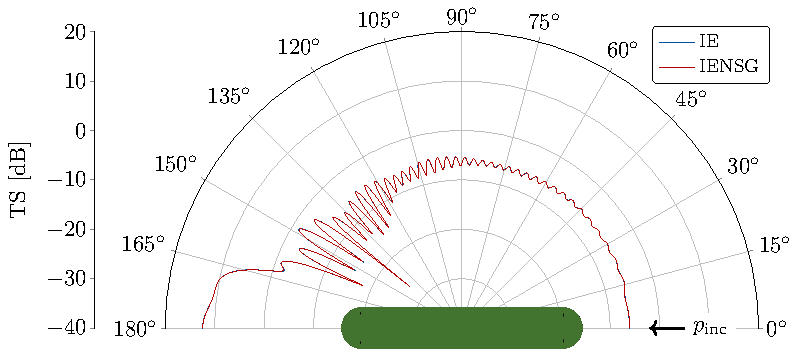
\includegraphics[width=\textwidth]{Shirron_5}
	\caption{\textbf{Shirron's mock shell}: Bistatic scattering on the mock shell with $\alpha_{\mathrm{s}} = \ang{0}$ and $\beta_{\mathrm{s}} = \ang{0}$ at $ka=10$ (where $a=\SI{1}{m}$ is the radius of the hemispherical endcaps).}
	\label{Fig3:Shirron}
\end{figure}
Results for the BeTSSi model 1 is produced in a similar fashion in~\Cref{Fig3:M1_IENSG_100} (with $\Gamma$ represented by \num{38414} dofs), illustrating very good results even if the infinite elements are attached directly onto the non-smooth scatterer using only $N=3$ basis functions in the radial direction. However, the results diverges at $f=\SI{1}{kHz}$ as illustrated in~\Cref{Fig3:M1_IENSG_1000}.
\begin{figure}
	\centering
	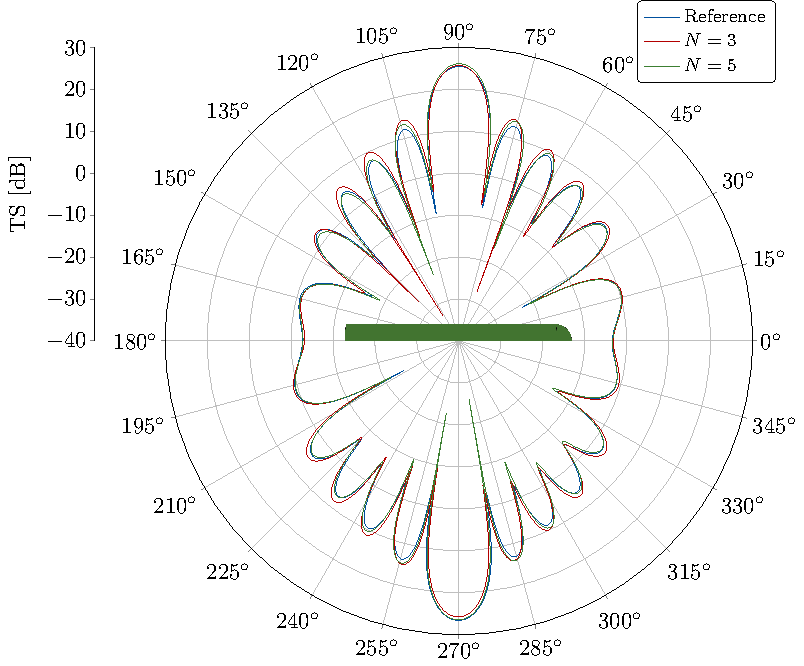
\includegraphics[width=\textwidth]{M1_100}
	\caption{\textbf{BeTSSi model 1}: Monostatic scattering at $f=\SI{100}{Hz}$ and $c_{\mathrm{f}}=\SI{1500}{m/s}$.}
	\label{Fig3:M1_IENSG_100}
\end{figure}
\begin{figure}
	\centering
	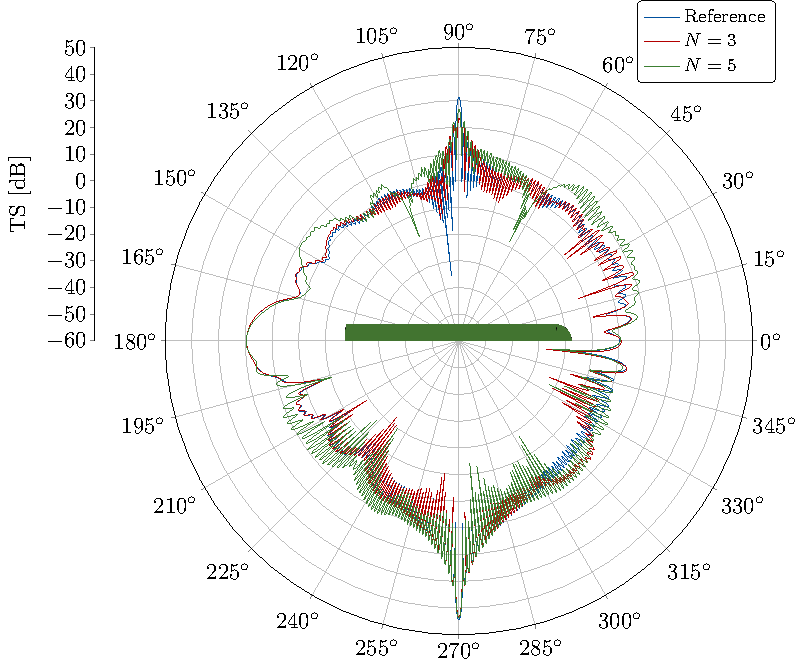
\includegraphics[width=\textwidth]{M1_1000}
	\caption{\textbf{BeTSSi model 1}: Monostatic scattering at $f=\SI{1000}{Hz}$ and $c_{\mathrm{f}}=\SI{1500}{m/s}$.}
	\label{Fig3:M1_IENSG_1000}
\end{figure}
%
%By defining
%\begin{align*}
%	K_{nm}^{(1)}(\vartheta,\varphi) &= \sum_{\tilde{n}=1}^N\sum_{\tilde{m}=1}^N\left[-2k^2r_{\mathrm{a}}^2B_{\tilde{n}+\tilde{m}}^{(1)} - \imag kr_{\mathrm{a}}(\tilde{n}+\tilde{m}+2)B_{\tilde{n}+\tilde{m}+1}^{(1)} + \left[\tilde{m}(\tilde{n}+2) +k^2\Upsilon^2\right]B_{\tilde{n}+\tilde{m}+2}^{(1)} \phantom{\left(\pderiv{r_{\mathrm{a}}}{\varphi}\right)^2} \right.\\
%	 &\left.{\hskip5em\relax}+ \imag k\frac{\Upsilon^2}{r_{\mathrm{a}}}(\tilde{n}+\tilde{m}+2)B_{\tilde{n}+\tilde{m}+3}^{(1)} - \frac{\tilde{m}(\tilde{n}+2)\Upsilon^2}{r_{\mathrm{a}}^2} B_{\tilde{n}+\tilde{m}+4}^{(1)}+k^2\Upsilon^2\cos^2\vartheta B_{\tilde{n}+\tilde{m}+2}^{(1)}\right. \\
%	 &\left.{\hskip5em\relax}+\frac{1}{r_{\mathrm{a}}}\left(\pderiv{r_{\mathrm{a}}}{\vartheta}\right)^2\left(k^2r_{\mathrm{a}}^2- \imag kr_{\mathrm{a}}(\tilde{n}+\tilde{m}+2)+ \tilde{m}(\tilde{n}+2)\right)\right.\\
%	 &\left.{\hskip11em\relax}\cdot\left(B_{\tilde{n}+\tilde{m}+2}^{(1)} + \frac{1}{\sin^2\vartheta}B_{\tilde{n}+\tilde{m}+1}^{(2)}-\frac{\Upsilon^2}{r_{\mathrm{a}}^2}\frac{\cos^2\vartheta}{\sin^2\vartheta} B_{\tilde{n}+\tilde{m}+3}^{(2)}\right)\right]\tilde{D}_{n\tilde{n}} D_{m\tilde{m}}
%\end{align*}
%\begin{align*}
%	K_{nm}^{(2)}(\vartheta,\varphi) &= \sum_{\tilde{n}=1}^N\sum_{\tilde{m}=1}^N B_{\tilde{n}+\tilde{m}+2}^{(1)}\tilde{D}_{n\tilde{n}} D_{m\tilde{m}}\\
%	K_{nm}^{(3)}(\vartheta,\varphi) &= \sum_{\tilde{n}=1}^N\sum_{\tilde{m}=1}^N \left(-\imag k + \frac{\tilde{m}}{r_{\mathrm{a}}}\right)B_{\tilde{n}+\tilde{m}+2}^{(1)}\tilde{D}_{n\tilde{n}} D_{m\tilde{m}}\\
%	K_{nm}^{(4)}(\vartheta,\varphi) &= \sum_{\tilde{n}=1}^N\sum_{\tilde{m}=1}^N \left(-\imag k + \frac{\tilde{n}+2}{r_{\mathrm{a}}}\right)B_{\tilde{n}+\tilde{m}+2}^{(1)}\tilde{D}_{n\tilde{n}} D_{m\tilde{m}}\\
%	K_{nm}^{(5)}(\vartheta,\varphi) &= \sum_{\tilde{n}=1}^N\sum_{\tilde{m}=1}^N \left(B_{\tilde{n}+\tilde{m}+1}^{(2)} - \frac{\Upsilon^2}{r_{\mathrm{a}}^2}\cos^2\vartheta B_{\tilde{n}+\tilde{m}+3}^{(2)}\right)\tilde{D}_{n\tilde{n}} D_{m\tilde{m}}\\
%	K_{nm}^{(6)}(\vartheta,\varphi) &= \sum_{\tilde{n}=1}^N\sum_{\tilde{m}=1}^N \left(-\imag k + \frac{\tilde{m}}{r_{\mathrm{a}}}\right)\left(B_{\tilde{n}+\tilde{m}+1}^{(2)} - \frac{\Upsilon^2}{r_{\mathrm{a}}^2}\cos^2\vartheta B_{\tilde{n}+\tilde{m}+3}^{(2)}\right)\tilde{D}_{n\tilde{n}} D_{m\tilde{m}}\\
%	K_{nm}^{(7)}(\vartheta,\varphi) &= \sum_{\tilde{n}=1}^N\sum_{\tilde{m}=1}^N \left(-\imag k + \frac{\tilde{n}+2}{r_{\mathrm{a}}}\right)\left(B_{\tilde{n}+\tilde{m}+1}^{(2)} - \frac{\Upsilon^2}{r_{\mathrm{a}}^2}\cos^2\vartheta B_{\tilde{n}+\tilde{m}+3}^{(2)}\right)\tilde{D}_{n\tilde{n}} D_{m\tilde{m}}\\
%\end{align*}
%we can write
%\begin{align*}
%	 K(\vartheta,\varphi) &= \left\{R_IR_J K_{nm}^{(1)} + \pderiv{R_I}{\vartheta}\pderiv{R_J}{\vartheta} K_{nm}^{(2)}+ \pderiv{r_{\mathrm{a}}}{\vartheta}\left(\pderiv{R_I}{\vartheta}R_JK_{nm}^{(3)} +R_I\pderiv{R_J}{\vartheta}K_{nm}^{(4)}\right) \right.\\
%	 &\left.{\hskip2em\relax}+\pderiv{R_I}{\varphi}\pderiv{R_J}{\varphi}\frac{1}{\sin^2\vartheta}K_{nm}^{(5)} + \pderiv{r_{\mathrm{a}}}{\varphi}\frac{1}{\sin^2\vartheta}\left(\pderiv{R_I}{\varphi}R_JK_{nm}^{(6)} +R_I\pderiv{R_J}{\varphi}K_{nm}^{(7)}\right)\right\}r_{\mathrm{a}}\euler^{-2\imag kr_{\mathrm{a}}}
%\end{align*}
%\subsection{Parametrization on a prolate ellipsoid for ABC operators}
%We typically parameterize the domain such that the artificial boundary $\Gamma$ is parameterized by $\xi$ and $\eta$. As $\vartheta = \vartheta(\xi,\eta)$ and $\varphi = \varphi(\xi,\eta)$ we have
%\begin{equation}
%	\diff \vartheta\diff\varphi = \begin{vmatrix}
%		\pderiv{\vartheta}{\xi} & \pderiv{\vartheta}{\eta}\\
%		\pderiv{\varphi}{\xi} & \pderiv{\varphi}{\eta}		
%	\end{vmatrix}\diff\xi\diff\eta
%\end{equation}
%where
%\begin{align*}
%	\pderiv{\vartheta}{\xi} &= \pderiv{\vartheta}{x}\pderiv{x}{\xi} + \pderiv{\vartheta}{y}\pderiv{y}{\xi} + \pderiv{\vartheta}{z}\pderiv{z}{\xi},\qquad
%	\pderiv{\vartheta}{\eta} = \pderiv{\vartheta}{x}\pderiv{x}{\eta} + \pderiv{\vartheta}{y}\pderiv{y}{\eta} + \pderiv{\vartheta}{z}\pderiv{z}{\eta}\\
%	\pderiv{\varphi}{\xi} &= \pderiv{\varphi}{x}\pderiv{x}{\xi} + \pderiv{\varphi}{y}\pderiv{y}{\xi} + \pderiv{\varphi}{z}\pderiv{z}{\xi},\qquad
%	\pderiv{\varphi}{\eta} = \pderiv{\varphi}{x}\pderiv{x}{\eta} + \pderiv{\varphi}{y}\pderiv{y}{\eta} + \pderiv{\varphi}{z}\pderiv{z}{\eta}
%\end{align*}
%and the inverse partial derivatives with respect to the coordinate transformation\footnote{From the prolate spheroidal coordinate system to the Cartesian coordinate system.\label{Fn:CartToProl}} are found in \Cref{Eq:dProlateSphericalCoordinatesdX}. This Jacobian matrix may be evaluated by
%\begin{equation*}
%	\vec{J}_3 = \begin{bmatrix}
%		\pderiv{\vartheta}{\xi} & \pderiv{\vartheta}{\eta}\\
%		\pderiv{\varphi}{\xi}	 & \pderiv{\varphi}{\eta}
%	\end{bmatrix} = \begin{bmatrix}
%		\pderiv{\vartheta}{x} & \pderiv{\vartheta}{y} & \pderiv{\vartheta}{z}\\
%		\pderiv{\varphi}{x} & \pderiv{\varphi}{y} & \pderiv{\varphi}{z}
%	\end{bmatrix}\begin{bmatrix}
%		\pderiv{x}{\xi} & \pderiv{x}{\eta}\\
%		\pderiv{y}{\xi} & \pderiv{y}{\eta}\\
%		\pderiv{z}{\xi} & \pderiv{z}{\eta}
%	\end{bmatrix}
%\end{equation*}
%and the derivatives of the basis functions may be computed by
%\begin{equation*}
%	\begin{bmatrix}
%		\pderiv{R_A}{\vartheta}\\
%		\pderiv{R_A}{\varphi}
%	\end{bmatrix} = \vec{J}_3^{-\transpose}\begin{bmatrix}
%		\pderiv{R_A}{\xi}\\
%		\pderiv{R_A}{\eta}	
%	\end{bmatrix}.
%\end{equation*}


%We typically parameterize the domain such that the artificial boundary $\Gamma_{\mathrm{a}}$ is parameterized by $\xi$ and $\eta$ at $\zeta=1$ (which is at $r=r_{\mathrm{a}}$ in the prolate spheroidal coordinates). As $\Gamma_{\mathrm{a}}$ is a surface with constant radius, $r=r_{\mathrm{a}}$, in the prolate spheroidal coordinate system, it may also be parametrized by $\vartheta$ and $\varphi$. We therefore have
%\begin{equation}
%	\diff \vartheta\diff\varphi = \begin{vmatrix}
%		\pderiv{\vartheta}{\xi} & \pderiv{\varphi}{\xi}\\
%		\pderiv{\vartheta}{\eta} & \pderiv{\varphi}{\eta}		
%	\end{vmatrix}\diff\xi\diff\eta
%\end{equation}
%where
%\begin{align*}
%	\pderiv{\vartheta}{\xi} &= \pderiv{\vartheta}{x}\pderiv{x}{\xi} + \pderiv{\vartheta}{y}\pderiv{y}{\xi} + \pderiv{\vartheta}{z}\pderiv{z}{\xi},\qquad
%	\pderiv{\vartheta}{\eta} = \pderiv{\vartheta}{x}\pderiv{x}{\eta} + \pderiv{\vartheta}{y}\pderiv{y}{\eta} + \pderiv{\vartheta}{z}\pderiv{z}{\eta}\\
%	\pderiv{\varphi}{\xi} &= \pderiv{\varphi}{x}\pderiv{x}{\xi} + \pderiv{\varphi}{y}\pderiv{y}{\xi} + \pderiv{\varphi}{z}\pderiv{z}{\xi},\qquad
%	\pderiv{\varphi}{\eta} = \pderiv{\varphi}{x}\pderiv{x}{\eta} + \pderiv{\varphi}{y}\pderiv{y}{\eta} + \pderiv{\varphi}{z}\pderiv{z}{\eta}
%\end{align*}
%and the inverse partial derivatives with respect to the coordinate transformation (from the prolate spheroidal coordinate system to the Cartesian coordinate system) is found in \Cref{Eq:dProlateSphericalCoordinatesdX}. The entries may be collected in a Jacobian matrix given by
%\begin{equation*}
%	J_3 = \begin{bmatrix}
%		\pderiv{r}{\xi}	 & \pderiv{r}{\eta} & \pderiv{r}{\zeta}\\
%		\pderiv{\vartheta}{\xi} & \pderiv{\vartheta}{\eta} & \pderiv{\vartheta}{\zeta} \\
%		\pderiv{\varphi}{\xi}	 & \pderiv{\varphi}{\eta} & \pderiv{\varphi}{\zeta}\\
%	\end{bmatrix} = \begin{bmatrix}
%		\pderiv{r}{x} & \pderiv{r}{y} & \pderiv{r}{z}\\
%		\pderiv{\vartheta}{x} & \pderiv{\vartheta}{y} & \pderiv{\vartheta}{z}\\
%		\pderiv{\varphi}{x} & \pderiv{\varphi}{y} & \pderiv{\varphi}{z}
%	\end{bmatrix}\begin{bmatrix}
%		\pderiv{x}{\xi} & \pderiv{x}{\eta} & \pderiv{x}{\zeta}\\
%		\pderiv{y}{\xi} & \pderiv{y}{\eta} & \pderiv{y}{\zeta}\\
%		\pderiv{z}{\xi} & \pderiv{z}{\eta} & \pderiv{z}{\zeta}
%	\end{bmatrix}
%\end{equation*}
%and the derivatives of a basis function $R$ may then be computed by
%\begin{equation*}
%	\begin{bmatrix}
%		\pderiv{R}{r}\\
%		\pderiv{R}{\vartheta}\\
%		\pderiv{R}{\varphi}
%	\end{bmatrix} = J_3^{-\transpose}\begin{bmatrix}
%		\pderiv{R}{\xi}\\
%		\pderiv{R}{\eta}	\\
%		\pderiv{R}{\zeta}	
%	\end{bmatrix}.
%\end{equation*}
%
%
%\begin{equation*}
%	\pderiv{R}{\xi} = \pderiv{R}{r}\pderiv{r}{\xi} + \pderiv{R}{\vartheta}\pderiv{\vartheta}{\xi} + \pderiv{R}{\varphi}\pderiv{\varphi}{\xi},\qquad
%	\pderiv{R}{\eta} = \pderiv{R}{r}\pderiv{r}{\eta} + \pderiv{R}{\vartheta}\pderiv{\vartheta}{\eta} + \pderiv{R}{\varphi}\pderiv{\varphi}{\eta},\qquad
%	\pderiv{R}{\zeta} = \pderiv{R}{r}\pderiv{r}{\zeta} + \pderiv{R}{\vartheta}\pderiv{\vartheta}{\zeta} + \pderiv{R}{\varphi}\pderiv{\varphi}{\zeta}
%\end{equation*}
%\begin{equation*}
%	\pderiv{R}{r} = \pderiv{R}{\xi}\pderiv{\xi}{r} + \pderiv{R}{\eta}\pderiv{\eta}{r} + \pderiv{R}{\zeta}\pderiv{\zeta}{r},\qquad
%	\pderiv{R}{\vartheta} = \pderiv{R}{\xi}\pderiv{\xi}{\vartheta} + \pderiv{R}{\eta}\pderiv{\eta}{\vartheta} + \pderiv{R}{\zeta}\pderiv{\zeta}{\vartheta},\qquad
%	\pderiv{R}{\varphi} = \pderiv{R}{\xi}\pderiv{\xi}{\varphi} + \pderiv{R}{\eta}\pderiv{\eta}{\varphi} + \pderiv{R}{\zeta}\pderiv{\zeta}{\varphi}
%\end{equation*}
%Thus,
%\begin{equation*}
%	\pderiv[2]{R}{r} = \pderiv{R}{y}
%\end{equation*}
